\chapter{Grundlagen und Methoden} 
In diesem Abschnitt werden die verwendeten Grundlagen und Methoden, die für die Umsetzung dieses Diplomarbeitsprojekts notwendig sind, dargestellt. Falls bei der Umsetzung mehrere Möglichkeiten zur Wahl standen, werden die einzelnen Möglichkeiten miteinander verglichen und nach einem Vergleich wird die besser geeignete Variante ausgewählt.


\section{Analyse des vorhandenen Systems}
Das bestehende System des Auftraggebers umfasst die Komponenten Grafana Server, Webserver und eine Datenbank mitsamt den notwendigen Algorithmen, um diese mit Echtzeitdaten zu befüllen. Bei der vorgegebenen Datenbank handelt es sich um einen MariaDB SQL-Server in der Version 10.1.48. Bei MySQL handelt es sich um eine quelloffene Implementierung des SQL Standards in der Version 5.0.12. In der nachfolgende Abbildung ist das vorhandene System des Auftraggebers ersichtlich.
\newline

\begin{figure}[h]
	\centering
	
\includegraphics[height=3cm,width=10cm]{images/vorhandeneSystemAuftraggeber}
	\caption{vorhandeneSystemAuftraggeber}
	\label{fig:vorhandeneSystemAuftraggeber}
\end{figure}
Der Grafana Server wird übernommen, um Dashboards für die Energiesysteme und Panels für die Energietechnologien zu erstellen. Dabei können mehrere Statistiken, auch Panels genannt, zu einem Dashboard zusammengefasst werden, um somit eine Ordnerstruktur am Grafana Server zu erlangen. Der Webserver wird als Produktivserver benützt, um die fertige Website zu präsentieren. Die vorhandene Datenbank wird aufgrund deren Schemas nicht übernommen, stattdessen wird ein neues besseres Datenbankschema entwickelt. Die dafür notwendigen Algorithmen, um die neue Datenbank mit Echtzeitdaten zu befüllen, werden vom Auftraggeber entwickelt.



\subsection{Begriffe}
In diesem Abschnitt werden notwendige Begriffe, die in dieser Diplomarbeit eine wichtige Rolle spielen und zu Missverständnissen führen könnten, erklärt.

\subsubsection{Echtzeitdaten} \label{sec:Echtzeitdaten}
Der Begriff Echtzeitdaten ist definiert durch die regelmäßige und in gleichen Zeitabständen erfolgende Erfassung sowie Verarbeitung von Daten einer Energietechnologie. Der Zeitabstand der Datenerfassung bei den Energietechnologien beträgt 30 Sekunden. Aufgrund des vorgegebenen Zeitabstandes werden die Echtzeitdaten als weiche Echtzeitanforderung definiert, da das Produkt alle einkommenden Daten schnellstmöglich mit einem konstanten Zeitabstand von 30 Sekunden bearbeitet. Ein Überschreiten dieser Zeitgrenze wird nicht als Versagen definiert, solange sich die Zeit noch in einem akzeptablen Toleranzbereich von wenigen Sekunden befindet. Eine Unterschreitung der Zeitangabe ist sehr selten möglich.  


\subsubsection{Energietechnologie} \label{sec:Energietechnologie}
Als Energietechnologie wird ein Stromerzeuger, Stromverbraucher oder ein Energiespeicher bezeichnet. Stromerzeuger sind PV-Anlagen oder Windkraftanlagen. Stromverbraucher sind E-Ladestationen oder Hausanschlusszähler. Batteriespeicher oder Wärmespeicher sind Speicher-Energietechnologien. Die von diesen Technologien erfassten Echtzeitdaten werden in einer Datenbank gespeichert und anschließend grafisch in Form von Statistiken visualisiert.

Dabei werden folgende Echtzeitdaten für die Statistiken verwendet:

\begin{itemize}
	\item Erzeuger/Verbraucher - Leistung [kW]
	\item Erzeuger/Verbraucher - Energie [kW/h]
	\item Speicher – Kapazität/Temperatur [kW/h]/[°]
\end{itemize}

Die folgende Tabelle bietet eine Übersicht aller vorhandenen Energietechnologien.
In der ersten Spalte der Tabelle befinden sich reine Erzeuger-Energietechnologien[PM1] . Verbraucher-Energietechnologien sind in der zweiten Spalte ersichtlich. Speicher-Energietechnologien in der dritten Spalte und in der vierten und zugleich auch letzten Spalte befinden sich Energietechnologien, die sowohl als Verbraucher-Energietechnologie und als Erzeuger-Energietechnologie definiert sind.
\begin{table}[]
	\begin{tabular}{|l|l|l|l|}
		\hline
		\textbf{Erzeuger} &\textbf{Verbraucher}  & 	\textbf{Speicher}            &  \textbf{Verbraucher \& Erzeuger}           \\ \hline
		PV-Anlage                   & Wasserstoff- Elektrolyse    & Batteriespeicher     & Biomasseheizkraftwerk             \\ \hline
		Stromnetzbezug              & E-Ladestation               & Wasserstoff-speicher & Biomasseheizwerk                  \\ \hline
		Wasserstoff Brennstoffzelle & Hausanschlusszähler         & Wärmespeicher        & Biomassekessel                    \\ \hline
		Windkraftanlage             & Gebäude- Wärmebedarfszähler & Kältespeicher        & Kompressionskältemaschine         \\ \hline
		Wärmenetzbezug              & Gebäude- Kältebedarfszähler &                      & Ab- oder \newline \\ &&&Adsorptionskältemaschine \\ \hline
		Solarthermieanlage          &                             &                      &                                   \\ \hline
		Wärmepumpe                  &                             &                      &                                   \\ \hline
	\end{tabular}
\caption{Energietechnologien}
\label{tab:Energietechnologien}
\end{table}


\newpage
\subsubsection{Energiesystem} \label{sec:Energiesystem}
Der Begriff Energiesystem fasst mehrere Energietechnologien in einem bestimmten Gebiet, die genau einem Energiesystem zugeordnet sind, logisch zusammen. Ein Energiesystem kann somit eine Gemeinde, ein Gebäude oder ein einziger Haushalt mit mehreren Energietechnologien sein.


\subsubsection{Front-End} \label{sec:Front-End}
Der Begriff Front-End beschreibt die Weboberfläche auf welcher der Benutzer verschiedene Interaktionen durchführen kann. Dabei umfasst dieser Begriff alle Unterseiten der Weboberfläche welche von einem Benutzer verwendet werden können.


\subsubsection{Back-End} \label{sec:Back-End}
Mit dem Begriff Back-End ist das Laravel-Projekt, welches für die Ereignisse der Benutzer-Interaktionen zuständig ist, gemeint. Zusätzlich sind in diesem Begriff die Zugriffe auf die Datenbank sowie auf den Grafana Server mit eingebunden, welche durch das Laravel-Projekt durchgeführt werden.

\section{Anforderungen an das Produkt}
Die Datenbank des Auftraggebers ist die größte Schwachstelle des vorhanden Systems.
Aufgrund dessen wird ein neues Datenbankschema entwickelt. Neben der Entwicklung eines neuen Datenbankschemas sind folgende Anforderungen an das Produkt gegeben:

\begin{itemize}
	\item Übersichtliche Darstellung von Energiesystemen und Energietechnologien auf einem Kartendienst
	\item Grafana-Statistiken mit Echtzeitdaten der Energietechnologien anzeigen
	\item Bildergalerie um Energietechnologien eines ausgewählten Energiesystems zu präsentieren
	\item Managementfunktion mit Hilfe von verschiedenen Benutzern für unterschiedliche Berechtigungen
\end{itemize}


\subsection{Schutz von vertraulichen Informationen}
Sämtliche Daten wie Adressen, Standorte (in Form von Koordinaten) oder die Namen der Ersteller von Energiesystemen oder Energietechnologien sind vertrauliche Informationen und sollten somit nicht für jeden einsehbar sein. Darum sind diese Daten nur in der Datenbank gespeichert, welche nur für Benutzer mit entsprechender Berechtigung zugänglich ist. Die Daten, die in den Grafana-Statistiken dargestellt werden, sind ebenso vertrauliche Daten. Die Informationen, die man einer solchen Statistik entnehmen kann, könnten in die falschen Hände gelangen und zu unerwünschten Tätigkeiten führen. Um dieses zu verhindern, sieht jeder angemeldete Benutzer nur seine eigenen Statistiken und keine anderen. Ein nicht angemeldeter Besucher sieht keine Statistiken.


\subsection{Statistische Auswertung}
Text



\section{Architektur des Zielsystems}
Die \autoref{fig:Architektur} repräsentiert die Architektur des Zielsystems. Der Benutzer greift über die Weboberfläche auf den Webserver zu, wo sich das Laravel-Projekt befindet. Auf dieser Website kann der Benutzer verschiedene Interaktionen durchführen. Dabei ist die Weboberfläche ständig in Verbindung mit der Datenbank sowie dem Grafana Server. Sobald der Benutzer auf die Energiesysteme-Seite der Weboberfläche wechselt, wird eine Datenbankabfrage aller vorhandenen Energiesysteme durchgeführt. Zusätzlich dazu wird mittels API-Abfrage auf den Grafana Server zugegriffen, um Statistiken einer Energietechnologie anzuzeigen, falls dies vom Benutzer angefordert wird.

\begin{figure}[h]
	\centering
	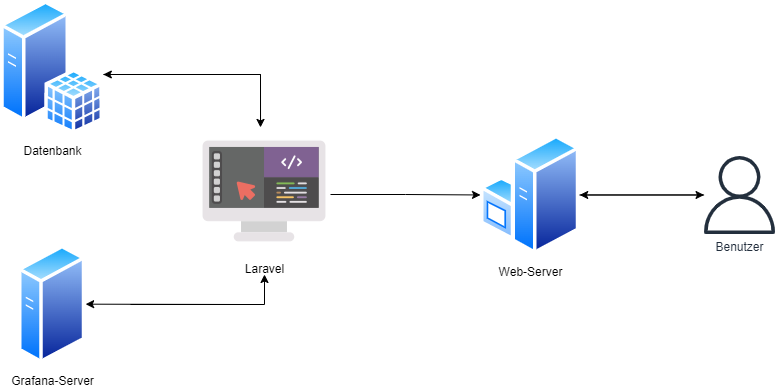
\includegraphics[height=8cm,width=15cm]{images/Architektur}
	\caption{Architektur}
	\label{fig:Architektur}
\end{figure}

\subsection{Endgeräte}
Das Produkt wurde als Browser Anwendung entwickelt, um überall lauffähig zu sein. Es ist in Chrome, Firefox und Edge Browser getestet worden und ist dort voll funktionsfähig. Die Oberfläche wurde für einen 13 bis 27 Zoll Monitor entwickelt und funktioniert dort in jeder Zoomstufe einwandfrei. Klares Ziel war es, das Produkt nicht für den Mobiltelefongebrauch zu programmieren. Bewusst wurde sich gegen eine native Anwendungsentwicklung entschieden, um so die Verwendbarkeit auf allen Plattformen zu garantieren. Darüber hinaus würde eine parallele Anwendungsentwicklung auf den drei gängigen Betriebssystemen (Windows, MacOS, Linux) den zeitlichen Rahmen der Diplomarbeit sprengen. Getestet wurde das Produkt in den Versionen:

\begin{itemize}
	\item Chrom 99.0.4844.51
	\item Firefox 98.0
	\item Edge 99.0
\end{itemize}

\subsection{Serverseitig}
Text

\subsection{Clientseitige Interaktion des Benutzers}
Bei dem Punkt Clientseitig befindet man sich in der Architektur des Zielsystems bei dem Element JavaScript und mit den damit verbundenen Interaktionen des Benutzers. Map-Interaktionen sind Interaktionen mit einer Karte, dazu gehört das Erstellen, Bearbeiten und Löschen von Energiesystemen sowie Energietechnologien. Eine weitere Interaktion wäre die Verwendung des Adresssuchfeldes, welche mit einem Klick auf den Button „Suche“ oder durch Drücken der Enter-Taste durchgeführt wird. Tabellen-Interaktionen sind eine zusätzliche clientseitige Aktion, da die vom DataTable\footnote{Eine genaue Begriffserklärung befindet sich in \ref{sec:DataTable}} bereitgestellten Funktionen wie die Suchfunktion, Sortierfunktion oder Seitennummerierung allesamt clientseitig stattfinden und somit keinen Einfluss auf das Back-End haben.
Folgende Abbildung zeigt den Aufbau der einzelnen Elemente, die zusammenarbeiten, um die Website zu erstellen.


\begin{figure}[h]
	\centering
	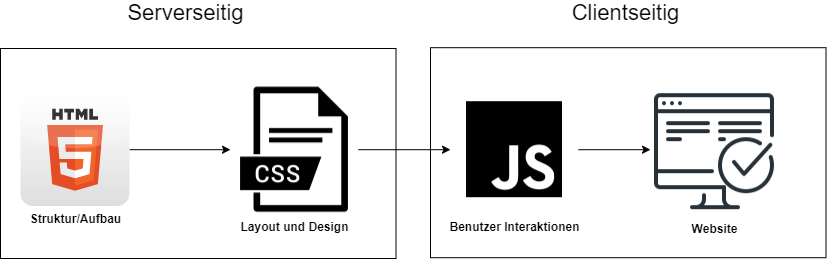
\includegraphics[height=4cm,width=12cm]{images/clientseitig}
	\caption{clientseitig}
	\label{fig:clientseitig}
\end{figure}

\subsection{Framework}
Die Wahl des Frameworks ist für die Umsetzung des Projekts entscheidend. Unter dem Begriff Framework versteht man eine Art Programmiergerüst, die es dem Programmierer deutlich erleichtert, ein Produkt zu erstellen. Jedes Framework bietet spezielle Lösungen und Lösungsansätze an und damit hat jedes einzelne sein eigenes Einsatzgebiet. In den nachfolgenden Unterkapiteln werden mögliche Frameworks für die Umsetzung des Projekts kurz erklärt. In \ref{sec:Entscheidung des Frameworks} wird genauer darauf eingegangen, welches Framework gewählt wurde und aus welchem Grund.

\subsubsection{Laravel}
Das PHP-Framework Laravel, welches 2011 entwickelt wurde, basiert auf dem MVC Muster\footnote{wird in  \autoref{sec:MVC} genauer erläutert} und bietet damit eine sehr gute Strukturierung und Übersicht beim Arbeiten. Laravel wird in den meisten Fällen als Back-End Framework verwendet. Die meisten Projekte werden mit Laravel im Back-End in Kombination mit Vue.js im Front-End umgesetzt. Genauere Informationen  zu Vue.js sind im Kapitel 2.6.3 nachzulesen. Laravel bietet jedoch die Möglichkeit, im Back- als auch im Front-End verwendet zu werden. Es lässt sich in folgende Einzelteile strukturieren:

\begin{itemize}
	\item Migrations 
	\item Views
	\item Controller 
	\item Models
	\item Routen 
\end{itemize}

Migrations sind die Abbildung der Tabellenstruktur und ermöglichen es, bei richtiger .env Datei Konfiguration, mit artisan Befehlen, ganz einfach eine Datenbank und die dazugehörigen Tabellen zu erstellen und diese auch genauso einfach wieder zu löschen oder zu leeren. Views fungieren als visueller Gliederungspart zwischen den Controllern und den Benutzern. In ihnen wird alles, was auf der Oberfläche ersichtlich ist, ausprogrammiert und gestaltet. Controller bilden die Verbindung zwischen den Views und den Models und ermöglichen es dem Benutzer, Daten mithilfe eines Zugriffs auf das Models zu verändern. Models bilden die Datenstruktur ab und ermöglichen den Zugriff auf die Daten und die Änderung dieser. Routen vermitteln die Benutzerabfrage von der View mit dem dazugehörigen Controller und werden in der Datei “web.php” definiert. Der ganze Prozess ist in \autoref{fig:Laravel MVC} visuell dargestellt. 
\begin{figure}[h]
	\centering
	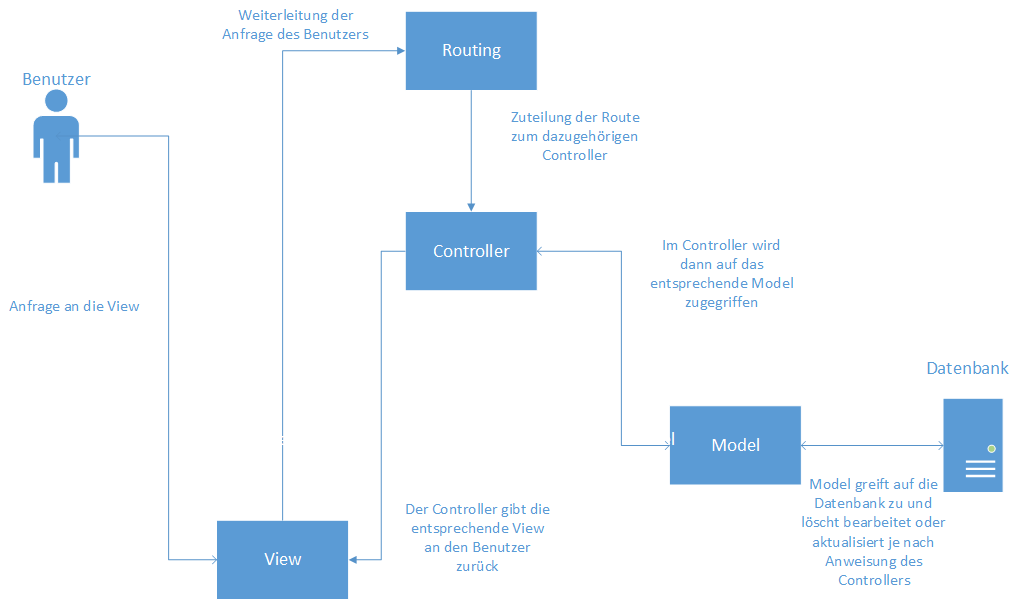
\includegraphics[height=8cm,width=15cm]{images/LaravelMVC}
	\caption{Laravel MVC}
	\label{fig:Laravel MVC}
\end{figure}
\newpage




\subsubsection{Angular}
Angular ist ein clientseitiges JavaScript-Web-Framework und wird meistens zum Erstellen von sogenannten Single Page Applications, wie beispielsweise ein einfaches Bedienelement zur Steuerung einer Maschine, verwendet. Angular ist speziell für Web-,Desktop- und Mobile-Anwendungen entworfen. Ein weiterer Aspekt des Frameworks ist es, dass es von Google entwickelt wurde, und so ein langfristiger Support gewährleistet ist. Angular macht es mit der Kombination aus HTML und TypeScript möglich, so ziemlich jede mögliche Aufgabenstellung zu bewältigen. Es bietet auch besondere Features wie eine bidirektionale Datenbindung an und ist somit gut für Echtzeitanwendungen geeignet. 
Weitere Informationen zu Angular können unter der Qulle xy (https://angular.de/artikel/was-ist-angular/) nachgelsen werden.
\begin{figure}[h]
	\centering
	
\includegraphics[height=6cm,width=8cm]{images/Angular_Logo}
	\caption{Angular Logo}
	\label{fig:Angular Logo}
\end{figure}
\newpage
\subsubsection{ASP.NET}
ASP.NET (Active Server Pages) ist ein Web Applications Framework, welches 2002 von der Firma Microsoft veröffentlicht wurde. Es ist der Nachfolger des ASP Frameworks und bietet eine perfekte Grundlage, um dynamische Websites, Webanwendungen und Webservices zu entwickeln. Projekte werden hier in der Regel in der Sprache C\# programmiert. Jedoch besteht auch die Möglichkeit, andere Sprachen wie beispielsweise Perl, Python oder Cobol zu verwenden. ASP.NET bietet nicht nur die Möglichkeit dynamische Websites zu erstellen, sondern auch Desktop Anwendungen.
Durch die vordefinierte Datenstruktur, die ASP.NET bereitstellt, hilft es dem Programmierer Programmiersprachen nicht zu vermischen und einen übersichtlichen Programmierstil beizubehalten. Des Weiteren können viele Teile automatisch generiert werden und ersparen dem Programmierer damit einen immensen Aufwand.

\begin{figure}[h]
	\centering
	
\includegraphics[height=6cm,width=8cm]{images/ASP.net_Logo}
	\caption{ASP.net Logo}
	\label{fig:ASP.net Logo}
\end{figure}


Genaure Informatione zu ASP.Net können unter der Quelle xy (https://asp.mvc-tutorial.com/de/421/einfuhrung/was-ist-asp-net-mvc/) nachgelesen werden.
\subsubsection{React}
React ist eine JavaScript-Softwarebibliothek, die es erleichtert, Benutzeroberflächen in Form von Web Applikationen zu erstellen. Es ist komponentenbasiert, was bedeutet, dass jedes Element in Blöcken aufgebaut ist und durch Zusammenfügen dieser einzelnen Codebits kann dann eine sogenannte View erstellt werden. Dies bietet die Möglichkeit, bereits erstellte Codebits auch in anderen Views zu verwenden. React wird oft zusammen mit ASP.NET verwendet.


Genaueres zu React kann unter der Quelle xy (https://t3n.de/news/react-facebook-623999/) nachgelesen werden.
\begin{figure}[h]
	\centering
	
\includegraphics[height=5cm,width=7cm]{images/React_Logo}
	\caption{React Logo}
	\label{fig:React Logo}
\end{figure}
\newpage

\subsubsection{Entscheidung des Frameworks}\label{sec:Entscheidung des Frameworks}
Positive und negative Aspekte jedes Framworks wurden vom Projektteam, mithilfe der Tabelle \ref{sec:Entscheidung des Frameworks}, abgewogen.

\begin{table}[h]
	
	\label{tab: Entscheidung des Frameworks}
	\begin{tabular}{|l|l|l|}
		\hline
		Framework &
		Vorteile &
		Nachteile \\ \hline
		React &
		\begin{tabular}[c]{@{}l@{}}Software Skalierbarkeit;\\ hohe Flexibilität;\\ Codebits ermöglichen es, die  Redundanz zu erhöhen; \\schnelles Rendering;\\ leichter Einstieg\end{tabular} &
		\begin{tabular}[c]{@{}l@{}}Es nicht genug Möglichkeiten,\\ eine Webapp zu erstellen \\ und benötigt Zusatzbibliotheken; \\ schweres debuggen;\\ komplexe Benutzeroberfläche\end{tabular} \\ \hline
		ASP.NET &
		\begin{tabular}[c]{@{}l@{}}hohe Flexibilität;\\ MVC Architektur; \\ gute Skalierbarkeit;\\ einfache Benutzung\end{tabular} &
		\begin{tabular}[c]{@{}l@{}}Ressourcenaufwendig;\\ Teuer aufgrund des Lizenskaufes;\\ keine aktuelle Dokumentation;\\alte Versionen sind nicht mehr kompatibel\end{tabular} \\ \hline
		Angular &
		\begin{tabular}[c]{@{}l@{}}frühzeitige Fehlererkennung;\\ Konsistent\end{tabular} &
		\begin{tabular}[c]{@{}l@{}}
		relativ starr und unflexibel;\\ schwer zu erlernen; 
	\end{tabular} \\ \hline
		 
		Laravel &
		\begin{tabular}[c]{@{}l@{}}Unit Tests werden angeboten;\\ einfache Erweiterbarkeit;\\ Routing in der App;\\ nutzt die neuesten Funktion von PHP;\\ sehr gute Dokumentation;\\ integrierte Benutzerverwaltung;\\ integrierte Mailverwaltung;\\ performant;\\ einfache Handhabung; \\ Bootstrap Einbindung ist einfach möglich\end{tabular} &
		\begin{tabular}[c]{@{}l@{}}unterstützt keine Zahlungsfunktion;\\ keine Mobil App Entwicklung;\\ oft Probleme bei Updates\end{tabular} \\ \hline
		
	\end{tabular}
	\caption{Entscheidung des Frameworks}
\end{table}
\newpage
Nach Begutachtung der Tabelle \ref{sec:Entscheidung des Frameworks} und aufgrund der überwiegenden positiven Aspekte , entschied sich das Projektteam für das Framework Laravel.Entscheidend war beispielsweise die einfache Handhabung und die Möglichkeit Bootstrap in Kombination zu verwenden. Da dieses Framework auch im Schulfach Softwareentwicklung genauer bearbeitet wurde, besitzt das Projektteam bereits ein gutes Grundwissen. Es wurde darüber hinaus überlegt, ob auch das Front-End Framework Vue.js zusätzlich verwendet werden soll. Da Vue.js nur zusätzliche Komplexität ohne einen wirklichen Nutzen mit sich bringen würde, wurde diese Option vernachlässigt. Das Framework Laravel bietet alle nötigen Front- und Back-End Möglichkeiten, die es ermöglichen, Laravel im Front wie auch im Back-End zu verwenden. Entscheidender Faktor war auch, dass das Projektteam noch nie mit einem anderen Framework gearbeitet hat, und so eigentlich nur Laravel in Frage gekommen ist.




\newpage
\subsection{Front-End Templates}
Die Auswahl des Front-End Templates ist essenziell für die Umsetzung der Weboberfläche des Produktes. Jedes Front-End Template bringt seine Vor- und Nachteile mit sich, wobei das Projektteam die Anforderungen an das Front-End Template mit den Vor- und Nachteilen jeden einzelnen Front-End Templates verglichen hat, um sich schlussendlich für eines zu entscheiden. Dabei sind die Anforderungen des Projektteams an das Front-End Template, dass es unkompliziert in das Projekt einzubinden ist und das Projektteam bereits Erfahrung damit hat, um das Arbeiten damit zu erleichtern. Weitere Anforderungen sind, dass es Responsive-Layouts ermöglicht, sowie Vorlagen von Komponenten, die eingebunden werden können, zur Verfügung stellt. Die drei Front-End Templates, die das Projektteam zur Auswahl stellt, sind Bootstrap, Tailwind und Vue.js.

\subsubsection{Bootstrap}
Bootstrap ist ein Open Source Front-End-CSS-Framework. Es basiert auf den Programmiersprachen HTML, CSS sowie JavaScript und stellt Gestaltungsvorlagen wie Formulare, Tabellen, Buttons und weitere Oberflächengestaltungen bereit. Bootstrap ist weltweit eines der bekanntesten und beliebtesten Front-End-Frameworks. Ebenso bietet Bootstrap eine Open Source-SVG-Icon-Bibliothek an, womit die Kompatibilität zwischen Komponenten und Icons bestenfalls gegeben ist. Vorteil dieses Templates ist, dass es leichtgewichtig ist, weil nur Front-End-Daten geladen werden müssen und keine Backend-Funktionalitäten. Zusätzlich ist es problemlos in das Projekt einzubinden und stellt mehrere Vorlagen zur Verfügung, die ebenso eingebunden werden können. Bootstrap ist kostenfrei zu verwenden, und das Projektteam bringt bereits Erfahrung mit diesem Template mit. Die Nachteile sind, dass Bootstrap wenige Back-End-Funktionen bereitstellt, und es ist weniger gut geeignet für sehr große Applikationen.
\newline
\begin{figure}[h]
	\centering
	
\includegraphics[height=8cm,width=10cm]{images/Bootstrap}
	\caption{Bootstrap Logo}
	\label{fig:Bootstrap Logo}
\end{figure}

\newpage
\subsubsection{Tailwind.css}
Tailwind ist ein Utility-First CSS-Framework, welches derzeit weltweit sehr beliebt ist. Diese Art von Framework soll mehr Flexibilität bieten als die traditionellen Vorgänger. Tailwind.css stellt Utility-Klassen zur Verfügung, mit denen man selbst Klassen zum Stylen der Komponenten definieren kann. Ein Inlinestylen ist bei diesem Framework ebenso möglich, womit externe CSS-Dateien überflüssig sind. Tailwind stellt Hilfsklassen zur Verfügung, welche das Arbeiten um einiges erleichtern. Zusätzlich bietet dieses Template eine hohe Flexibilität sowie mehrere Funktionen, um ein Responsive Design zu erreichen. Jedoch hat dieses Template keine vorgefertigten Komponenten, auf welche zurückgegriffen werden kann, und der Benutzer dieses Templates braucht sehr viel Zeit zum Erlernen der richtigen Verwendung. Die Größe der zu installierenden CSS-Datei ist sehr groß, da dieses Template eine breite Palette von Klassen bereitstellt, wobei die meisten oft in einem Projekt nicht verwendet werden. Das Projektteam hat mit diesem Template wenig Erfahrung, und die Dokumentation im Internet ist sehr mangelhaft.
\begin{figure}[h]
	\centering
	
\includegraphics[height=8cm,width=10cm]{images/Tailwind}
	\caption{Tailwind Logo}
	\label{fig:Tailwind Logo}
\end{figure}


\newpage
\subsubsection{Vue.js}
Das JavaScript Framework Vue.js, welches für die Front-End-Entwicklung eingesetzt werden kann, wird immer populärer. Die Einfachheit und Benutzerfreundlichkeit ist ein Grund für die immer größer werdende Beliebtheit. Vue.js basiert auf dem virtuellen DOM \footnote{Virtuelles Document Object Model, beim Aktualisieren schneller als das herkömmliche}, was bedeutet, dass das Abarbeiten von Befehlen schneller funktioniert als beim herkömmlichen bekannten DOM\footnote{Document Object Model, stellt XML oder HTML Dokumente als Baumstruktur dar}. Vue.js basiert auf den Programmiersprachen HTML, CSS und JavaScript, womit die wichtigsten verwendeten Sprachen abgedeckt sind. Vue.js stellt Funktionen wie UniTests, End-to-End-Tests sowie Routing-Systeme bereit. Die Lesbarkeit bei diesem Template ist sehr gut, da alle Komponenten sich in einer Datei befinden. Das Projektteam hat nur wenig Erfahrung mit diesem Template und es herrschen generelle Sprachbarrieren, da vieles nur in der Sprache Chinesisch vorhanden ist.
\begin{figure}[h]
	\centering
	
\includegraphics[height=6cm,width=8cm]{images/vuejs}
	\caption{Vuejs Logo}
	\label{fig:Vuejs Logo}
\end{figure}


\newpage
\subsubsection{Entscheidung des Front-End Templates}
Das Projektteam hat sich für das Front-End Template Bootstrap CSS entschieden aufgrund der Vorteile, die es mit sich bringt. Diese Entscheidung wurde unter anderem deswegen so getroffen, da das Projektteam bereits Erfahrung mit diesem Framework sammeln konnte und dieses Framework alle Anforderungen, die an das Front-End Template gestellt wurden, erfüllt.
In der nachfolgenden Tabelle ist eine Gegenüberstellung der Vor- und Nachteile der Front-End Templates ersichtlich:

\begin{table}[h]
	\begin{tabular}{|l|l|l|}
		\hline
		\textbf{Front-End Template} &\textbf{Vorteile}  & 	\textbf{Nachteile}    \\ \hline
		
		\textbf{Bootstrap}                   &
		
		basiert auf HTML, CSS und JavaScript & wenige Back-End Funktionen \\ 
		&
		stellt Gestaltungsvorlagen bereit 
		&   nicht geeignet für große Applikationen \\
	 &	weltweit sehr bekannt und beliebt&  \\
		&
		leicht in das Projekt einzubinden&  \\
		&
		Projektteam hat bereits Erfahrungen damit& 
		
		
		
		          \\ \hline
		          
		\textbf{Tailwind.css}        &
		 
		weltweit sehr beliebt & keine vorgefertigten Komponenten \\
		&
		bietet mehr Flexibilität & Projektteam hat sehr wenig Erfahrung \\
		&
		stellt Utility-Klassen zur Verfügung &  		  Online-Dokumentation ist mangelhaft \\
		& &  		  erfahrungsloser Benutzer  \\
		&&  		  benötigt viel Einarbeitungszeit\\
		&&		  Größe der CSS-Datei ist enorm \\
	
		       \hline
		      
		\textbf{Vue.js} &
		 einfach und benutzerfreundlich  & Projektteam hat wenig Erfahrung \\
		 &
		basiert auf HTML, CSS und JavaScript & 		 Sprachbarrieren, vieles nur auf Chinesisch \\
		&
		stellt Funktionen wie UniTests, & \\
		&
		 End-to-End Tests und & \\
		 &Routing-Systeme bereit  &  \\ 
		 &
		hohe Lesbarkeit des Codes & 
		
		                  \\ \hline
		                  
	\end{tabular}
	\caption{Vor- und Nachteile der Front-End Templates}
	\label{tab:Vor- und Nachteile der Front-End Templates}
\end{table}

\newpage
\subsection{Verbindung der Datenbank mit Laravel}
In Laravel ist die Verbindung  der Datenbank mithilfe der .env Datei möglich. Tabellen werden in sogenannten Migrations definiert. Auf die einzelnen Komponenten und deren Individualisierung wird in den Kapiteln \ref{sec:Laravel .env Datei} und \ref{sec:Migrations} noch genauer eingegangen.
\subsubsection{Laravel .env Datei } \label{sec:Laravel .env Datei}
In Laravel bietet die .env Datei, welche sich direkt im Projektordner befindet, die Möglichkeit, alle nötigen Umgebungsvariablen zu initialisieren. Ein Beispiel für Umgebungsvariablen sind Datenbank Anmeldeinformationen, Cache-Treiber, Mail-Server-Domain oder auch die App URL. Wichtig ist es, dass die .env Datei immer Gerät spezifisch konfiguriert wird. Das heißt, es ist wichtig beim Zusammenarbeiten, speziell mit Git, sehr gut aufzupassen. Folgedessen ist es empfehlenswert, die .env Datei  mit einem Gitignore\footnote{Gitignore gibt an, welche Datei bei einem Git Pull nicht heruntergeladen werden soll} zu versehen, um Komplikationen zu vermeiden. Es besteht auch die Möglichkeit,  Änderungen in der .env Datei direkt aus dem Programm vorzunehmen. 

\subsubsection{Migrations}\label{sec:Migrations}
Migrations bilden in Laravel eine Möglichkeit, die Tabellenstruktur im Programm selbst fest zu legen. Sie sind sozusagen der Blueprint\footnote{ein Blueprint ist sozusagen der Bauplan oder eine Vorlage wie etwas auszusehen hat}, in welchem die gesamte Tabellenstruktur vordefiniert ist. Für jede Tabelle, die in der Datenbank, welche vorher in der  .env Datei  definiert wurde, erstellt werden soll, gibt es eine eigene Migration. Migrations sind unterteilt in eine up() und in eine down()  Methode\footnote{Methoden sind ein Art Container für den in ihnen auszuführenden Code}. In der up() Methode wird der Name der Tabelle der Name der einzelnen Tupel und deren Datentyp definiert. Der Datentyp id() ist standardmäßig immer der primary Key. 
In der down() Methode wird die Tabelle von der Datenbank gelöscht. Die beiden Methoden werden durch artisan Befehle, welche im Kapitel 3.10 ersichtlich sind, angesteuert. 
Erstellt werden Migrations mithilfe eines weiteren Laravel Befehls, welcher ebenfalls  im Kapitel 3.10.1 beschrieben wird. Wenn die Migration erfolgreich erstellt wurde, ist diese folgendermaßen benannt : JJJJ.MM.DD\_tempname.php und befindet sich im Ordner Projektname\textbackslash database \textbackslash migrations.


Alle Informationen liegen der Quelle (https://laravel.com/docs/9.x/migrations) zugrunde.
\newpage
\subsubsection{Seeder und Factories}
Factories ermöglichen es,  Fake Models\footnote{Fake Models sind Models die nur temporär angelegt werden} zu erstellen und mithilfe dieser auf die Datensätze in der Datenbank  zuzugreifen und diese zu verändern. Daten werden mithilfe der Open Source-Bibliothek Faker generiert. Die Faker Bibliothek kann folgende Daten generieren: 



\begin{itemize}
	\item E-Mail 
	\item einen Namen
	\item eine Telefonnummer 
	\item Wörter
	\item Sätze 
	\item Absätze
	\item Zufallszahlen
\end{itemize}

Datenbank-Factories  erlauben es , Tabellen programmgesteuert mit Daten anzufüllen. Sie ermöglichen es, innerhalb von einigen Minuten tausende Daten in die Datenbank zu schreiben.
Die Hauptaufgabe eines Seeder ist es jedoch nur die Factories aufzurufen.

\subsubsection{Datenübergabe in Laravel}
Ein Controller hat die Aufgabe mithilfe eines Models die Daten zu verändern und danach eine View zurückzugeben. Möchte man jedoch Daten wie Attribute, welche im Formular mitgeschickt werden, auf der zurückgegebenen View verwenden, müssen diese mitgegeben werden.
Es gibt die Möglichkeit, Daten mithilfe von compact in das Return Statement\footnote{Rückgabewert einer Funktion}anzuhängen. Dies würde im Code folgendermaßen aussehen: 
\definecolor{mygray}{RGB}{252,251,244}
\renewcommand{\lstlistingname}{Quellcode}

\begin{lstlisting}[
	caption={Return Statemnet mit Compact},
	label=Code,
	language=octave,
	numbers=left,
	firstnumber=1,
	numberfirstline=false,
	backgroundcolor=\color{mygray},
	basicstyle=\footnotesize=15,
	keywordstyle=\color{blue}
	]
	return view(Viewname , compact('data'));
	
\end{lstlisting}

In der View kann dann mit folgendem Code auf die Daten zugegriffen werden:
\definecolor{mygray}{RGB}{252,251,244}
\renewcommand{\lstlistingname}{Quellcode}

\begin{lstlisting}[
	caption={Zugriff mittels Foreach Schleife},
	label=Code,
	language=octave,
	numbers=left,
	firstnumber=1,
	numberfirstline=false,
	backgroundcolor=\color{mygray},
	basicstyle=\footnotesize=15,
	keywordstyle=\color{blue}
	]
	@foreach ($data as $d)
	$d->Beispiel_Attribut 
	@endforeach
	
\end{lstlisting}

Die zweite Variante Daten zu Übergeben schaut folgendermaßen aus:
\definecolor{mygray}{RGB}{252,251,244}
\renewcommand{\lstlistingname}{Quellcode}

\begin{lstlisting}[
	caption={Attributübermittlung in einem return View Statment},
	label=Code,
	language=octave,
	numbers=left,
	firstnumber=1,
	numberfirstline=false,
	backgroundcolor=\color{mygray},
	basicstyle=\footnotesize=15,
	keywordstyle=\color{blue}
	]
return view('Viewname', ['AttributName' => 'AttributWert']);
\end{lstlisting}
\newpage

Diese Variante bietet den Vorteil, dass im Code gleich direkt auf das Attribut zugegriffen werden kann und keine  Foreach Schleife nötig ist. Ein solcher Zugriff würde folgendermaßen aussehen : 
\definecolor{mygray}{RGB}{252,251,244}
\renewcommand{\lstlistingname}{Quellcode}

\begin{lstlisting}[
	caption={Zugriff im Program},
	label=Code,
	language=octave,
	numbers=left,
	firstnumber=1,
	numberfirstline=false,
	backgroundcolor=\color{mygray},
	basicstyle=\footnotesize=15,
	keywordstyle=\color{blue}
	]
{{ $AttributName }}
\end{lstlisting}


Alle Informationen und Arten der Datenübergabe wurden aus dem Video aus der Quelle xy () entnommen.


\section {Visuelle Darstellung der Energiesysteme und Energietechnologien }
Von Seiten des Auftraggebers wurde von Anfang an der Wunsch geäußert, Energiesysteme und Energietechnologien, mithilfe eines Kartendienstes visuell darzustellen. Um andere Möglichkeiten, wie eine Karte auszuschließen, wurde auch zu Geoinformationssystem und CSS-System recherchiert. Die Ergebnisse dieser Recherchen werden in den nachfolgenden Kapiteln behandelt. 

\subsection{Kartendienste}
Das Produkt stellt eine zentrale Verwaltungsmöglichkeit in Form einer Karte bereit. Um diese Karte auf dem Produkt zu verwenden, wird ein Kartenanbieter benötigt. Die Zwei Optionen Google Maps und OpenStreetMap wurden vom Projektteam analysiert. Auf diese zwei Anbieter wird in den Kapitel \ref{sec:OpenStreetMap} und \ref{sec:Gooogle Maps} genauer eingegangen. Von Seiten des Auftraggebers wurde, aufgrund einer gewissen Abneigung zu Diensten, die von Google bereitgestellt werden, eine Präferenz zu OpenStreetMap geäußert.

\subsubsection{Google Maps} \label{sec:Gooogle Map}


Google Maps ist der klare Marktführer in der Sparte der Kartendienst Anbieter.  Der Großteil  aller Webanwendungen, welche Maps verwenden, werden mit Google Maps umgesetzt. Google Maps überzeugt nicht nur mit einer sehr hohen Individualisierungsmöglichkeiten, sondern auch mit einer sehr hohen Ausfallsicherheit. Der größte Vorteil ist jedoch, das große Angebot an vordefinierten Api Diensten. Diese können einfach über die Google Cloud Platform überwacht, bedient oder aktiviert werden. Genauere Infos zur Google Maps Plattform stehen im Kapitel 3.9. Ein weiterer Vorteil von Google Maps ist es, dass es wirklich weitflächig alles abdeckt, ganz im Gegensatz zu OpenStreetMap. Der einzige Nachteil ist, dass die Verwendung einer Google Maps Karte auf der Website kostenpflichtig ist. Es gibt jedoch auf der Google Cloud Seite eine genaue Kostenaufstellung. Bezahlt wird bei Verwendung der Api Dienste. Google verrechnet hier je nach Api Dienst einen gewissen Betrag pro Verwendung. Diese Kosten waren jedoch bei der Entwicklung kein Problem, da auf Google Cloud für die ersten 30 Tage ein Startkapital von 300 Dollar anbietet.  
\begin{figure}[h]
	\centering
	
\includegraphics[height=5cm,width=7cm]{images/GoogleMapsLogo}
	\caption{Google Maps Logo}
	\label{fig:GoogleMaps Logo}
\end{figure}
\newpage
\subsubsection{OpenStreetMap}\label{sec:OpenStreetMap}


OpenStreetMap ist ein 2004 gegründetes Projekt, welches das Ziel hat, eine frei verfügbare Weltkarte zu erstellen. Gegründet wurde dieses Projekt von Steve Coast und zählt mittlerweile um die 7.8 Millionen Nutzer. Das Hauptargument OpenStreetMap eher als Google Maps zu verwenden ist es, dass dieses kostenlos und lizenzfrei ist. Es gibt jedoch gravierende Nachteile gegenüber Google Maps. Openstreetmap bietet keine  Api Dienste an. Es gibt zwar die Möglichkeit, mithilfe von Leaflet, welches eine JavaScript-Bibliothek ist, eigenen Api Dienste zu programmieren, dies ist jedoch mit einem sehr hohen Aufwand und einer sehr hohen Komplexität verbunden. Ein weiterer Nachteil von Openstreetmap ist es, dass es auf Benutzerdaten aufbaut. Das bedeutet, Nutzer sind  dafür verantwortlich, die Karte immer auf dem aktuellsten Stand zu halten. Somit ist dieser Kartendienst wenig zuverlässig.
Ein weiterer Nachteil wäre, dass Daten für alle User zugänglich sind. 
\begin{figure}[h]
	\centering
	
\includegraphics[height=5cm,width=7cm]{images/OpenStreetMap_Logo}
	\caption{Open Street Map Logo}
	\label{fig:Open Street Map Logo}
\end{figure}

Informationen über OpenStreetMap wurden aus der Quelle xy () entnommen.
\newpage

\subsection{Geoinformationssystem }
Die aufwendigste Option ist es, die Energiesysteme mittels GPS (Global Positioning System) zu orten und diese dann auf der Seite visuell darzustellen. In diesem Falle müsste das Galileo, welches das Europäische GPS System ist, genutzt werden. Galileo ist ein offenes, kostenloses Signal, welches es ermöglicht, den Sender auf bis zu zwei Meter genau zu orten. Ein solcher GPS Sender würde auf circa zehn bis zwanzig Euro pro System oder Technologie kommen. Die gesendeten Signale können mithilfe eines Empfängers ausgewertet werden.

\subsection{CSS-System}
Eine weitere Option ist es, die Energiesysteme und Technologien mittels CSS auf der Website darzustellen. Eine Möglichkeit wäre es, die Koordinaten der Systeme in die Datenbank zu schreiben, diese dann in Laravel auszulesen und auf einem selbst erstellten Hintergrund  einzuzeichnen. Dieses System könnte in Kombination mit einem Geoinformationssystem * verwendet werden. Dies könnte dann folgendermaßen aussehen: 

\begin{figure}[h]
	\centering
	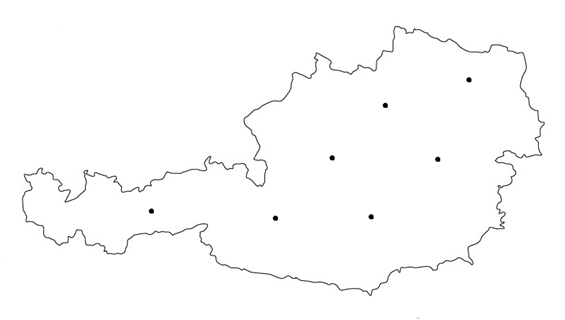
\includegraphics[height=6cm,width=10cm]{images/CSS_System}
	\caption{Beispiel eines CSS-Systems}
	\label{fig:CSS_System}
\end{figure}


\subsection{Auswahl des Anbieters}
	Bei der Wahl des Anbieters, müsste der Auftraggeber Best GmbH berücksichtigt werden. Folgende Punkte muss der Anbieter erfüllen:
	\begin{itemize}
		\item leichte Implementierung 
		\item es sollen alle gewünschten Funktionen umsetzbar sein 
		\item es soll möglichst ohne viel extra Aufwand möglich sein  
		\item es soll nicht Kostspielig sein 
	\end{itemize}

Um die Anbieter auf die gewünschten Anforderungen zu Überprüfen wurde die Liste angefertigt.

\begin{table}[h]

	\begin{tabular}{|l|l|l|l|l|}
		\hline
		Anbieter &
		Kosten &
		Apis vorhanden &
		Umsetzbarkeit(Zeit) &
		Vorteile und Nachteile \\ \hline
		Google Maps &
		gering &
		ja &
		ja &
		\begin{tabular}[c]{@{}l@{}}viele Apis,\\ die die Arbeit erleichtern;\\ einfache Einbindung auf der Website;\\ performant;\\ großflächig aufgeschlossen;\\ Daten nur für den\\ Betreiber selbst einsehbar\end{tabular} \\ \hline
		Open Street Map &
		keine &
		nein &
		nein &
		\begin{tabular}[c]{@{}l@{}}keine Apis vorhanden;\\ viel mehr Aufwand,\\ um das Gleiche wie\\ Google Maps zu bieten;\\ unperformant;\\ keine großflächige Aufschließung;\\ Daten sind für Jeden einsehbar\end{tabular} \\ \hline
		Geoinformationssystem &
		sehr hohe &
		nein &
		nein &
		\begin{tabular}[c]{@{}l@{}}genaue Ortung der Systeme;\\ sehr preisintensiv;\\ sehr zeitintensiv und komplex\end{tabular} \\ \hline
		CSS-System &
		keine &
		nein &
		ja &
		\begin{tabular}[c]{@{}l@{}}keine Apis;\\ sehr viel Aufwand;\\ erfüllt den gleichen Zweck \\wie eine Karte\end{tabular} \\ \hline
	\end{tabular}
\end{table}



\section{Berechtigungssystem Benutzer}
Im folgenden Abschnitt wird näher auf das Benutzerverwaltungssystem eingegangen sowie auf die vorhandenen Benutzerrollen, die einem Benutzer zugeteilt werden können.

\subsection{Benutzerrollen}
Die Weboberfläche bietet für deren Besucher ein rollenbasiertes Benutzersystem an, um die Funktionen für jeden Benutzer zu deklarieren.
Das rollenbasierte Benutzersystem unterscheidet zwischen folgenden Benutzern:

\begin{itemize}
	\item Administrator 
	\item Mitarbeiter
	\item Öffentlicher Benutzer 
\end{itemize}



\subsubsection{Administrator}
Der Administrator-Benutzer ist der höchste Benutzer von allen. Er darf Energiesysteme sowie Energietechnologien erstellen und alle anderen vorhandenen bearbeiten und löschen. Zusätzlich dazu hat er Einsicht in sämtliche Grafana-Statistiken. Diese Benutzerrolle hat das Recht, neue Benutzer auf der Weboberfläche zu registrieren und vorhandene zu löschen, was für alle anderen Benutzer nicht möglich ist.

\subsubsection{Mitarbeiter}
Die Rolle „Mitarbeiter“ darf auf der Weboberfläche neue Energiesysteme sowie Energietechnologien erstellen. Die von ihm erstellten Energiesysteme sowie Energietechnologien kann er bearbeiten oder  löschen, und er hat auf diesen ebenso die Berechtigung auf Einsicht der Statistiken. Andere Mitarbeiter dürfen seine Energiesysteme und Energietechnologien nicht bearbeiten oder löschen und haben keinen Zugriff auf dessen Statistiken mit Ausnahme des Administrators. Ein Mitarbeiter-Benutzer darf somit nur seine selbst erstellten Energiesysteme und Energietechnologien verwalten. Der Mitarbeiter-Benutzer hat nicht die Berechtigung, neue Benutzer zu registrieren oder vorhandene zu löschen.

\subsubsection{öffentlicher Benutzer}
Dieser Benutzer hat die geringste Berechtigung und tritt in Kraft, wenn man nicht auf der Weboberfläche angemeldet ist. Dieser Benutzer darf keine Energiesysteme sowie Energietechnologien erstellen, bearbeiten oder löschen. Zusätzlich hat der öffentliche Benutzer keine Einsicht auf sämtliche Grafana-Statistiken. Der Zugang zu der Benutzerverwaltung ist ebenso nicht erreichbar. Dieser Benutzer sieht lediglich die öffentlichen Daten, die für jedes Energiesystem und jede Energietechnologie preisgegeben werden.

\subsection{Berechtigungen in Laravel}
Im folgenden Abschnitt wird erklärt, wie in Laravel die zuvor genannten Benutzerrollen unterschieden werden.
Dafür bietet Laravel Authentifizierungsrichtlinien. Dabei kann mit den Befehlen @auth und @guest überprüft werden, ob der aktuelle Benutzer authentifiziert oder ein Gast ist. Je nach Authentifizierung und Rolle hat der Benutzer unterschiedliche Rechte sowie Funktionen zur Verfügung.
Für genauere Informationen, wie eine Berechtigungsüberprüfung in Laravel umgesetzt werden kann, siehe Quelle x.y.



\section{Ui/Ux Design}
Im Wort Ui/Ux Design steht das Ui für User Interface und Ux für User Experience. Es handelt davon, wie eine Website von einem Nutzer aufgefasst und wahrgenommen wird. Es beschreibt die Wirkung, die das Design auf einen Nutzer hat. Genauer beschreibt die User Experience wie sich ein Nutzer auf der Website fühlt oder wie er auf ihr navigieren kann. 
Ziel ist es, dem Benutzer ein möglichst entspanntes Gefühl zu geben und ihm bei Allem zu helfen. Das User Interface beschäftigt sich vielmehr mit der Website an sich. Man macht sich hierbei Gedanken, ob der Benutzer das Design ansprechend finden könnte, oder ob überall die idealen Elemente oder Elementgrößen gewählt wurden. Eine weitere Frage, die man sich im User Interface überlegt, ist was wirkt auf den Benutzer positiv was negativ. Einige Methoden das Ui/Ux Design umzusetzen sind : 

\begin{itemize}
	\item Erstellen eines Wireframes 
	\item Umfragen an Usern durchführen
	\item Fragebögen auf der Seite selbst 
	\item erstellen einer Übersicht mit den Anforderungen der Benutzer
\end{itemize}
Nützliche Programme zum Erstellen der besagten Dokumente  sind folgende : 
\begin{itemize}
	\item Kissmetrics
	\item Figma
	\item SimilarWeb
\end{itemize}

\subsection{Wireframe}
Ein Wireframe hilfe dem Design Team eine grobe Struktur der Website vorzudefinieren. Bei der Erstellung eines Wireframes wird der Visuelle Design Part komplett vernachlässigt. Bei einem Wireframe wird sich auf den Aufbau und die Position der Elemente konzentriert. Es ist meist in schwarz und weiß gehalten, da Farben bei diesem Aufbauprozess nur behindern würden. 
\subsection{Persona}
Eine Persona dient dazu, die Bedürfnisse und Ziele der Zielgruppe zu erfassen. Mit hilfe der Persona kann auf Wünsche und Bedürfnisse der Benutzer während der Entwicklung eingegangen werden. Empfohlen wird pro Zielgruppe um die fünf bis sechs Personen das Produkt testen zu lassen. Erstellt werden sie dann auf Grundlage von :
\begin{itemize}
	\item Interviews mit dem Benutzer
	\item Benutzertests
	\item Umfragen
\end{itemize}

\section{Template Layout}
Laravel bietet die Möglichkeit, mithilfe einer Layout Datei, Codeabschnitte auf mehreren Seiten zu verwenden. Hauptsächlich wird diese Funktion genutzt, um statische Elemente, die auf jeder Unterseite gleich sind, nur einmal zu programmieren. Ein gutes Beispiel wäre der Header oder auch der Footer, da sich diese Elemente auf den Unterseiten meist nicht variieren. 

\subsection{Platzhalter Yield}
In der Layout Datei kann \@yield verwendet werden, um Platz zu halten. Dies ermöglicht es, beispielsweise den Titel der Website individuell für jede Unterseite zu setzen. Der Platzhalter wird in der Layout Datei folgendermaßen konfiguriert:  <title>\@yield('title')</title> .  Möchte man diesen Platzhalter dann auf einer der Unterseiten, welche die Layout Datei verwenden, setzen, ist das folgendermaßen möglich : \@section('title', 'titlename'). Das Projektteam verwendet dieses Statement auf jeder Unterseite, um den Titel zu setzen.

\subsection{Sections}
Sections ermöglichen es, die Layout Datei in Abschnitte zu unterteilen. Der Beginn einer Section wird mit dem Befehl: \@section('sectionname) gekennzeichnet. Um die Section wieder zu schließen, muss folgendes Statement benutzt werden: \@endsection. Die Einteilung des Codes in Section erlaubt es, dieses Codestück auf einer anderen Seite mit nur einem Stichwort einzubinden. 
\subsection{Einbindung der definierten Sections}
Um diese im Layout File definierten Sections im Code einbinden zu können, müssen einige Einstellungen vorgenommen werden. Am Anfang einer neuen Seite muss dieser Code eingefügt werden: \@extends('layoutfilenname'). Damit wird der Seite mitgeteilt, dass die angegebene Seite als Layout Vorlage verwenden werden soll. Wenn diese Zeile vorhanden ist, können mittels\@section('sectioname') die im Layout File definierten Sections eingebunden werden. Wichtig ist,  jedesmal nach dem \@section auch ein \@endsection einzugeben, sonst wird die Section nicht angezeigt. Zur Ergänzung der Section kann man den zu ergänzenden Code einfach zwischen dem \@section und dem \@endsection platzieren. Dieser wird dann zum bereits vordefinierten Code ergänzt.

\section{Laravel Befehle}
Laravel bietet die Möglichkeit, viele Dinge mithilfe der Konsole Models,Controller oder Views, automatisch generieren zu lassen. In den folgenden Unterkapiteln werden die Wichtigsten dieser Befehle aufgelistet und kurz erklärt.
\subsection{Migration Befehle}
Um eine neue Migration zu erstellen, muss folgendes Kommando in der Commandline ausgeführt werden:
\definecolor{mygray}{RGB}{252,251,244}
\renewcommand{\lstlistingname}{Quellcode}

\begin{lstlisting}[
	caption={Erstellen einer neuen Migration},
	label=Code,
	language=octave,
	numbers=left,
	firstnumber=1,
	numberfirstline=false,
	backgroundcolor=\color{mygray},
	basicstyle=\footnotesize=15,
	keywordstyle=\color{blue}
	]
php artisan make:migration migration_name
\end{lstlisting}
Wenn die Migration erfolgreich erstellt und initialisiert wurde, kann man mit folgendem Kommando die up() Methode aller Migrations aufrufen:
\definecolor{mygray}{RGB}{252,251,244}
\renewcommand{\lstlistingname}{Quellcode}

\begin{lstlisting}[
	caption={Erstellen einer neuen Migration},
	label=Code,
	language=octave,
	numbers=left,
	firstnumber=1,
	numberfirstline=false,
	backgroundcolor=\color{mygray},
	basicstyle=\footnotesize=15,
	keywordstyle=\color{blue}
	]
	php artisan migrate
\end{lstlisting}
Nach Ausführung dieses Kommandos sind alle Tabellen in der Datenbank so wie gewünscht erstellt. 
Um alle ausgeführten Migrations anzeigen zu lassen, muss dieses Kommando verwendet werden:
\definecolor{mygray}{RGB}{252,251,244}
\renewcommand{\lstlistingname}{Quellcode}

\begin{lstlisting}[
	caption={Erstellen einer neuen Migration},
	label=Code,
	language=octave,
	numbers=left,
	firstnumber=1,
	numberfirstline=false,
	backgroundcolor=\color{mygray},
	basicstyle=\footnotesize=15,
	keywordstyle=\color{blue}
	]
php artisan migrate:status
\end{lstlisting}
Wenn die zuletzt erstellten Tabellen rückgängig gemacht werden sollen, gibt es die Möglichkeit, folgendes Kommando auszuführen:
\definecolor{mygray}{RGB}{252,251,244}
\renewcommand{\lstlistingname}{Quellcode}

\begin{lstlisting}[
	caption={Erstellen einer neuen Migration},
	label=Code,
	language=octave,
	numbers=left,
	firstnumber=1,
	numberfirstline=false,
	backgroundcolor=\color{mygray},
	basicstyle=\footnotesize=15,
	keywordstyle=\color{blue}
	]
	php artisan migrate:rollback 
\end{lstlisting}
Weitere nützliche Befehle sind unter  der Quelle xy () zu finden.

\subsection{Seeder und Factory Befehle}
Um einen Datenbank Seeder zu erstellen, ist folgendes Kommando notwendig: 
\begin{lstlisting}[
	caption={Erstellen einer neuen Migration},
	label=Code,
	language=octave,
	numbers=left,
	firstnumber=1,
	numberfirstline=false,
	backgroundcolor=\color{mygray},
	basicstyle=\footnotesize=15,
	keywordstyle=\color{blue}
	]
php artisan make:seeder seeder_name
\end{lstlisting}
Wenn eine Factory erstellt werden soll, gibt es folgende Möglichkeit:
\begin{lstlisting}[
	caption={Erstellen einer neuen Migration},
	label=Code,
	language=octave,
	numbers=left,
	firstnumber=1,
	numberfirstline=false,
	backgroundcolor=\color{mygray},
	basicstyle=\footnotesize=15,
	keywordstyle=\color{blue}
	]
	php artisan make:factory factory_name
\end{lstlisting}

Um den Seeder nach Initialisierung auszuführen, gibt es folgende Möglichkeit:
\begin{lstlisting}[
	caption={Erstellen einer neuen Migration},
	label=Code,
	language=octave,
	numbers=left,
	firstnumber=1,
	numberfirstline=false,
	backgroundcolor=\color{mygray},
	basicstyle=\footnotesize=15,
	keywordstyle=\color{blue}
	]
	php artisan db:seed
\end{lstlisting}
Weitere nützliche Befehle und Individualizations Möglichkeiten sind unter der Quelle xy() verzeichnet.
\subsection{Model und Controller Befehle}
Um ein neues Model zu erstellen, verwendet man dieses Kommando:
\begin{lstlisting}[
	caption={Erstellen einer neuen Migration},
	label=Code,
	language=octave,
	numbers=left,
	firstnumber=1,
	numberfirstline=false,
	backgroundcolor=\color{mygray},
	basicstyle=\footnotesize=15,
	keywordstyle=\color{blue}
	]
php artisan make:model model_name
\end{lstlisting}
Um einen normalen Controller anzulegen, gibt es folgendes Kommando:
\begin{lstlisting}[
	caption={Erstellen einer neuen Migration},
	label=Code,
	language=octave,
	numbers=left,
	firstnumber=1,
	numberfirstline=false,
	backgroundcolor=\color{mygray},
	basicstyle=\footnotesize=15,
	keywordstyle=\color{blue}
	]
	php artisan make:controller controller_name
\end{lstlisting}
Es gibt ergänzend die Möglichkeit, einen Resource Controller anzulegen. 
Ein Resource Controller hat den Vorteil, dass er vorgenerierte Methoden besitzt, wie zum Beispiel:
\begin{itemize}
	\item index()
	\item create()
	\item store()
	\item show()
	\item edit()
	\item update()
	\item destroy()
\end{itemize}
Erstellt wird ein Resource Controller folgendermaßen:
\begin{lstlisting}[
	caption={Erstellen einer neuen Migration},
	label=Code,
	language=octave,
	numbers=left,
	firstnumber=1,
	numberfirstline=false,
	backgroundcolor=\color{mygray},
	basicstyle=\footnotesize=15,
	keywordstyle=\color{blue}
	]
	php artisan make:controller controller_name --resource
\end{lstlisting}
Genauere Informationen zu der Erstellung von Models und Controllern finden sie unter der Quelle xy ().

\subsection{Starten des Laravel Develop Servers}
Laravel bietet die Möglichkeit, wenn PHP auf dem Entwicklungssystem installiert ist, einen PHP Development Server zu hosten und das Projekt über den Localhost anzuzeigen. Um den Server zu starten, muss folgende Zeile eingeben werden:
\begin{lstlisting}[
	caption={Erstellen einer neuen Migration},
	label=Code,
	language=octave,
	numbers=left,
	firstnumber=1,
	numberfirstline=false,
	backgroundcolor=\color{mygray},
	basicstyle=\footnotesize=15,
	keywordstyle=\color{blue}
	]
	php artisan serve
\end{lstlisting}
Nach Ausführen dieses Kommandos kann man das Projekt unter http://localhost:8000 aufgerufen werden.


\subsection{Befehle nach dem Git Pull} 
Bei Team Projekten in Laravel ist Git die beste Lösung. Jedoch kommt es oft zu Komplikationen beim Herunterladen des Projektes durch Git. Es gibt aber einige Befehle, die es ermöglichen, das Laravel Projekt komplikationsfrei zu starten.
Dieser Kommand sorgt dafür, dass der APP\_KEY in der .env Datei richtig gesetzt wird:
\begin{lstlisting}[
	caption={Erstellen einer neuen Migration},
	label=Code,
	language=octave,
	numbers=left,
	firstnumber=1,
	numberfirstline=false,
	backgroundcolor=\color{mygray},
	basicstyle=\footnotesize=15,
	keywordstyle=\color{blue}
	]
php artisan key:generate 

\end{lstlisting}
Um sicher zu stellen, dass alle nötigen Pakete installiert wurden, kann folgender Befehl verwendet werden:
\begin{lstlisting}[
	caption={Erstellen einer neuen Migration},
	label=Code,
	language=octave,
	numbers=left,
	firstnumber=1,
	numberfirstline=false,
	backgroundcolor=\color{mygray},
	basicstyle=\footnotesize=15,
	keywordstyle=\color{blue}
	]
	composer update
	
\end{lstlisting}
Nach Durchführung dieser Schritte sollte sich das Programm problemlos starten und verändern lassen.



\section{Routen in Laravel}
Laravel Verfügt über ein Ausgedehntes Routing System über welches Views aber auch ganze Gruppen von Elementen angesprochen und angezeigt werden können. Diese Routen werden in der Datei “web.php” angelegt und verwaltet.
\subsection{Ressource Routen} 
Mit der Ressource Route wird ein ganzer Controller angesprochen, so können über diese Route alle Methoden in diesem Controller angesprochen und verwendet werden. Im Produkt wird jeder Controller welcher wiederum für jede Tabelle vorhanden ist durch eine Ressource Route adressiert. Dieser Vorgang wird in Abbildung 2.14 veranschaulicht.

\begin{figure}[h]
	\centering
	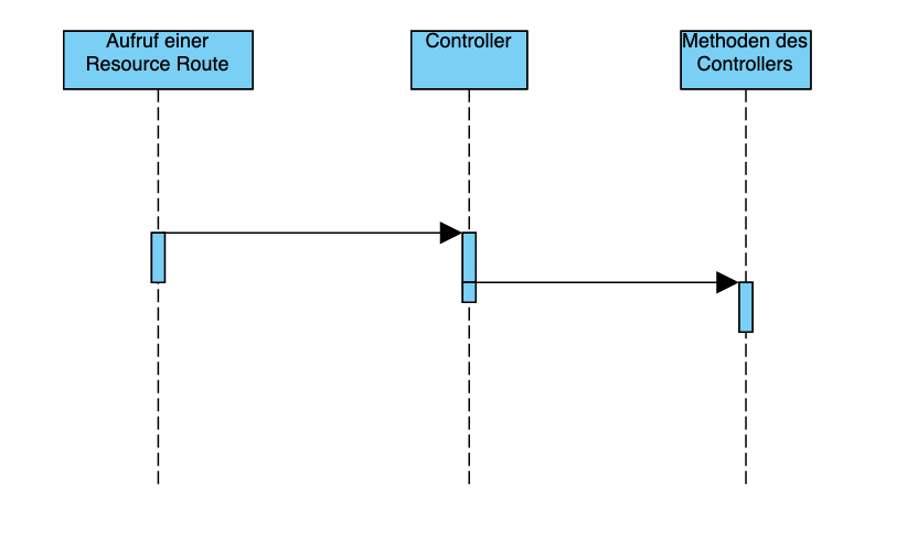
\includegraphics[height=6cm,width=9cm]{images/ResourceRoute}
	\caption{Aufbau einer Ressource Route}
	\label{fig:ResourceRoute}
\end{figure}

\subsection{GET Routen}
Mit diesem Typ von Routen lässt sich eine bestimmte Methode in einem ausgewählten Controller adressieren. Außerdem ist es möglich in einer GET Route einen Parameter mitzugeben welcher dann in der ausgewählten Methode im Controller verarbeitet wird. Im Produkt werden dieser Typ von Methoden verwendet um beispielsweise die Startseite anzuzeigen. Weiters werden sie verwendet um bestimmte Methoden in Controllern zB. löschen von Energiesystemen mit der Id des ausgewählten Objektes auszuführen. Am meisten kommt dieser Typ von Routen beim erstellen, editieren oder Löschen von Datenbankeinträgen zum Einsatz, da hier ein gewisser Eintrag mit dem mitgelieferten Parameter einer Route adressiert werden kann. Der Aufbau dieser Route wird in Abbildung 2.15 verdeutlicht.

\newpage
\begin{figure}[h]
	\centering
	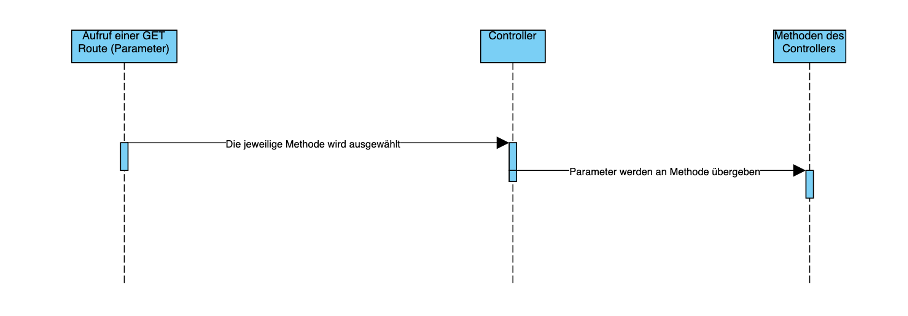
\includegraphics[height=6cm,width=16cm]{images/GETRoute}
	\caption{Aufbau einer GET Route}
	\label{fig:GETRoute}
\end{figure}

\subsection{Auth Routen}
Sobald in Laravel das Authentifizierungssystem aktiviert wird werden diese Routen automatisch erstellt. Diese Routen adressieren die ebenfalls durch Laravel erstellen auth Controller in der die Benutzeranmeldung sowie Registrierung bearbeitet wird.

\section{MVC}
Das Produkt verwendet das von Laravel bereitgestellte Design Pattern MVC (Model, View, Controller) welches in der Abbildung 2.16 Dargestellt wird. 

\begin{figure}[h]
	\centering
	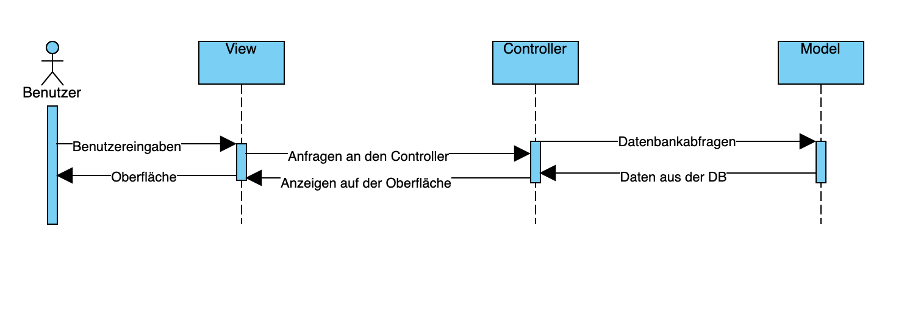
\includegraphics[height=6cm,width=18cm]{images/MVC}
	\caption{MVC Design Pattern}
	\label{fig:MVC}
\end{figure}

\subsection{Model}
Für jede durch eine Migration (Kapitel 3.2.2)  erstellte Tabelle gibt es ein Model, in diesem wird wie der Name suggeriert das Datenmodell abgebildet. Durch diesen Ansatz kann von jedem Model eine Instanz erstellt werden und so die Entsprechende Tabelle in einem beliebigen Programmabschnitt verwendet werden. Weiters werden in den Models die Relationen zwischen den einzelnen Tabellen beschrieben.
\subsection{View}
Das Produkt baut auf 8 Views auf in diesen Views werden die Daten welche von den Controllern übergeben werden mithilfe von Datatables (Kapitel 3.6) dem User angezeigt. Weiters gibt es in den Views verschiedene Möglichkeiten der User interaktion.
\subsection{Controller}
In den Controllern wird der Datenweg zwischen den Views also den User Interaktionen und der Datenbank gesteuert. Für jede durch eine Migration in der Datenbank erstelle Tabelle gibt es einen Controller welcher das Speichern, die Ausgabe, das Editieren sowie das Löschen von einzelnen Tupeln aus der Datenbank steuert. Weiters werden in den store und destroy Methoden des EnTechControllers sowie des EnSysControllers die Api Aufrufe an die Grafana http Api mit den vom User eingegebenen Daten ausgeführt.

\chapter{Ergebnisdokumentation }
Dieser Abschnitt beinhaltet eine Dokumentation der verwendeten Werkzeuge zur Umsetzung der einzelnen Funktionen. Es werden alle behandelten Teilbereiche erläutert.

\section{Laravel }
In diesem Kapitel werden die Ereignisse und Erfahrungen dokumentiert welche sich im laufe der Produktentwicklung mit dem Laravel Framework herausgestellt haben.

\subsection{Installation}
Die Installation von Laravel erfolgt mithilfe des PHP Installations Tool Composer. Composer installiert hierzu die Paketquellen Lokal auf dem System. Beim Erstellen eines neuen Laravel Projektes werden die von Composer installierten Quelldateien in das Verzeichnis des neu zu erstellenden Projektes kopiert und installiert. Im nachfolgenden Link ist mehr über die Installation von Laravel zu lesen:
\href{https://laravel.com/docs/9.x#installation-via-composer}{Dokumentation der Installation}


\subsection{Bootstrap Einbindung}
Für das Design des Frontends wird die CSS Bibliothek “Bootstrap” (Kapitel 2.3.6.1) verwendet, hierzu werden die Quelldateien von Bootstrap durch Composer lokal abgespeichert und durch den Laravel Befehl "php artisan ui bootstrap“ dem Laravel Projekt hinzugefügt. Laravel bietet die Möglichkeit beim hinzufügen von Bootstrap mit der Option “-- auth” direkt die Beispielseiten (Login, Registrieren) für den Authentifizierungsvorgang zu erstellen. Im nachfolgenden Link ist mehr über die Installation von Bootstrap zu lesen:
\href{https://www.positronx.io/how-to-properly-install-and-use-bootstrap-in-laravel/}{Dokumentation der Installation}


\subsection{Grafana Einbindung}
Text

\subsection{MVC}\label{sec:MVC}
Text
\subsubsection{Model}
Text
\subsubsection{View}
Text
\subsubsection{Controller}
Text


\section{Datenbankanbindung in Laravel}
Um die Datenbank an das Programm anzubinden, müssen einige Änderungen in der .env Datei vorgenommen werden. Genauere Information zur .env Datei befinden sich im Kapitel  2.3.9.1. Welche Konfigurationen genau getätigt werden, können in den nachfolgenden Kapiteln nachgelesen werden. 

\subsection{Datenbank Anmeldeinformationen}
Eine Änderung war es, die Datenbank Anmeldeinformationen auf die richtigen Einstellungen zu setzen. Es können folgende Parameter gesetzt werden : 
\begin{itemize}
	\item DB\_CONNECTION
	\item DB\_HOST
	\item DB\_PORT
	\item DB\_DATABASE
	\item DB\_USERNAME
	\item DB\_PASSWORD
\end{itemize}

DB\_CONNECTION symbolisiert die Zugriffsvariante auf die Datenbank. DB\_HOST bezeichnet die Domain des Datenbankservers, beispielsweise 127.0.0.1, wenn der Datenbankserver über den Localhost bereitgestellt wird. DB\_PORT ist dementsprechend der Port, auf welchem die Datenbank erreichbar ist. DB\_DATABASE ist der Name der Datenbank, auf die zugegriffen werden soll. DB\_USERNAME der Benutzername, mit welchem man auf die Datenbank zugreifen möchte. Diese Einstellungen sind vom Projekt Team vorgenommen worden, um eine Datenbank verwenden zu können und diese löschen beziehungsweise erstellen zu können.
\subsection{Mail Server Konfigurationen}
Um auf der Weboberfläche das Passwort Resetten mittels E-Mail zu ermöglichen, muss Laravel eine E-Mail versenden. Dazu braucht es die nötigen Konfigurationen in der .env Datei. Folgende Attribute müssen gesetzt werden: 
\begin{itemize}
	\item MAIL\_MAILER
	\item MAIL\_HOST 
	\item MAIL\_PORT 
	\item MAIL\_USERNAME 
	\item MAIL\_PASSWORD
	\item MAIL\_ENCRYPTION 
	\item MAIL\_FROM\_ADDRESS
	\item MAIL\_FROM\_NAME 
\end{itemize}
Bei MAIL\_MAILER wird das Protokoll eingetragen. Bei MAIL\_HOST wird die Host Domain  eingegeben, also welcher SMTP Server verwendet werden soll. MAIL\_PORT gibt an, unter welchem Port der Server erreicht werden soll. MAIL\_USERNAME: hier muss die E-Mail Adresse, welche zum Absenden der Mail verwendet wird, eingetragen werden. Beim MAIL\_PASSWORD muss das dazugehörige Passwort eingetragen werden. MAIL\_ENCRYPTION gibt an, mit welchem Verfahren verschlüsselt werden soll. MAIL\_FROM\_ADDRESS ist die Adresse, welche beim Empfänger als Sender E-Mail angezeigt wird. MAIL\_FROM\_NAME ist der Name der beim Empfänger angezeigt wird. Das Produkt verwendet diese Einstellungen um eine Passwort Reset Email an den Benutzer zu senden. Alle geforderten Einstellungen wurden nach Übergabe an den Auftraggeber von diesem Konfiguriert. 
\subsection{Migrations}
Die Migrations wurden dazu verwendet, um Tabellen zu gestalten. In ihnen wurden alle nötigen Attributnamen und deren Datentypen konfiguriert. Das Produkt verwendet folgende von Laravel automatisch erzeugte Migrations für die Benutzerauthentifizierung: 
\begin{itemize}
\item 2014\_10\_12\_000000\_create\_users\_table.php
\item 2014\_10\_12\_100000\_create\_password\_resets\_table.php
\item 2019\_08\_19\_000000\_create\_failed\_jobs\_table.php
\item 2019\_12\_14\_000001\_create\_personal\_access\_tokens\_table.php
\end{itemize}
Zusätzlich zu diesen bereits erstellten Migrations wurde für jede Energietechnologieart eine eigene Migration angelegt. Darüber hinaus wurden Templates\footnote{ein Template ist ein Grundbauplan} für ein Energiesystem und eine Energietechnologie erstellt. Im Energietechnologien Template sind alle Attribute, die bei jeder Energietechnologie gleich sind. Alle individuellen Attribute werden dann mithilfe der eigener Migrations abgebildet.
\newpage
\section{Routen in Laravel}
Text

\subsection{Resource Routen}
Text

\subsection{GET Routen}
Text

\subsection{Auth Routen}
Text


\section{Datenbankdesign}
Text

\subsection{Erstellen eines neuen Schemas}
Text

\subsubsection{ER-Model}
Text

\subsubsection{Fremdschlüssel}
Text


\section{Corporate Design}
Vom Projektteam wurde ein Corporate Design Manual erstellt. Dieses befindet sich auch auf der DVD der Diplomarbeit. In diesem Corporate Design Manual wurden folgende Themen bearbeitet: 
\begin{itemize}
	\item Oberfläche
	\item Definierte Farben
	\item Verwendung der definierten Farben
	\item Überschriften
	\item Buttons 
	\item Interaktionsfarben
	\item Schriftarten
	\item Schriftgrade
	\item Logo
	\item Verwendete Icons
	\item Bedeutung der Icons 
	\item Icons mit Funktionalitäten 	
	\item Website Design

\end{itemize}
Auf die wichtigsten Elemente wird in den nachfolgen Kapiteln eingegangen.
\subsection{Vorschläge}
Nach Absprache der Grundanforderung des Produktes wurden, mithilfe der Adobe xd Software,  drei Designvorschläge verfasst. Diese sind auch auf der DVD der Diplomarbeit einsehbar. Um diese aussagekräftig zu vergleichen, wird von jedem Vorschlag, in den nachfolgenden drei Abbildungen, die Energiesystem Seite visuell dargestellt.
\begin{figure}[h]
	\centering
	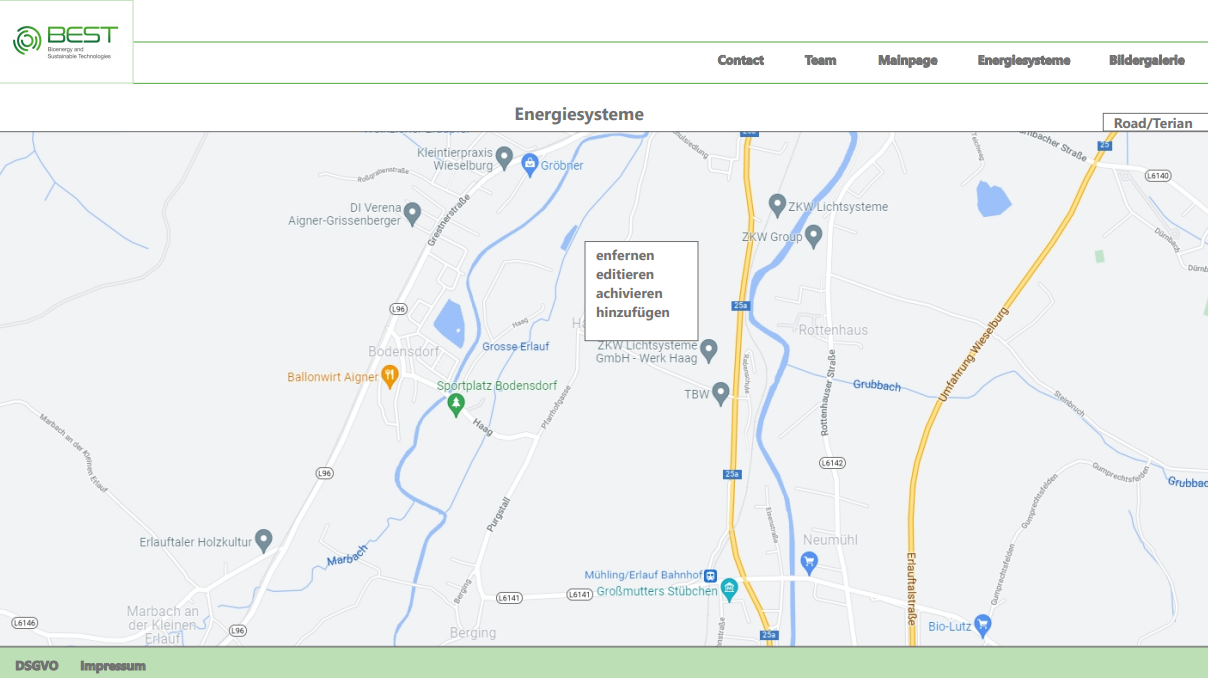
\includegraphics[height=6cm,width=12cm]{images/DesignVorschlag1}
	\caption{Design Vorschlag 1}
	\label{fig:Design Vorschlag 1}
\end{figure}
\newpage
\begin{figure}[h]
	\centering
	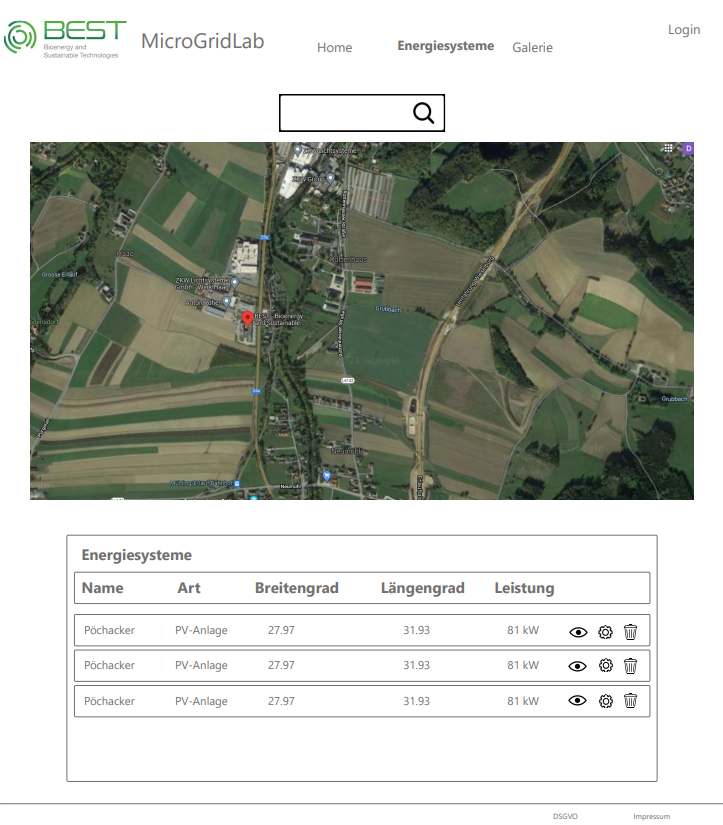
\includegraphics[height=12cm,width=11cm]{images/DesignVorschlag2}
	\caption{Design Vorschlag 2}
	\label{fig:Design Vorschlag 2}
\end{figure}
\begin{figure}[h]
	\centering
	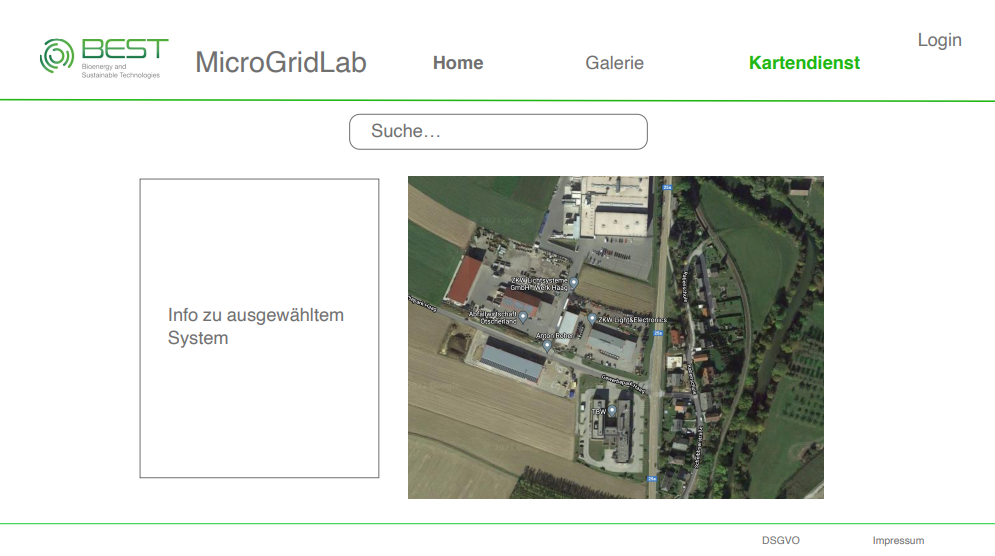
\includegraphics[height=7cm,width=12cm]{images/DesignVorschlag3}
	\caption{Design Vorschlag 3}
	\label{fig:Design Vorschlag 3}
\end{figure}
\subsection{Änderungsvorschläge} \label{sec:Änderungsvorschläge}
Die oben ersichtlichen Design Vorschläge wurden dem Auftraggeber über Skype präsentiert. Dieser favorisierte die Vorschläge \ref{fig:Design Vorschlag 1} und  \ref{fig:Design Vorschlag 2}. 
Von Seiten des Auftraggebers kamen viele Verbesserungsvorschläge und Ideen. Einige davon sind:
\begin{itemize}
	\item Die Liste soll neben der Map platziert werden.
	\item Es soll folgende Unterseiten geben:
	\subitem Home
	\subitem Energiesysteme
	\subitem Galerie
	\item Es soll Icons geben, welche es ermöglichen, Energiesysteme und Energietechnologien in der Liste zu löschen, bearbeiten oder einzusehen. 
	\item Es sollen die Farben aus der CSS Datei der bereits vorhanden Website extrahiert werden.
	
\end{itemize}


\subsection{Finales Design}
Nach genauer Definition der Änderungsvorschläge in Kapitel \ref{sec:Änderungsvorschläge}, wurde erneut in Adobe XD ein Design Vorschlag erstellt. Dieser Vorschlag war eine Mischung aus dem Vorschlag 1 und dem Vorschlag 2 mit den gewünschten Änderungen des Auftraggebers. Auch dieser Vorschlag ist auf der DVD der Diplomarbeit einsehbar. Um einen Vergleich zwischen Vorschlag 1 , Vorschlag 2 und dem finalen Design zu ermöglichen, wird nachfolgend auch die Energiesystem Seite des finalen Vorschlags visuelle dargestellt.

\begin{figure}[h]
	\centering
	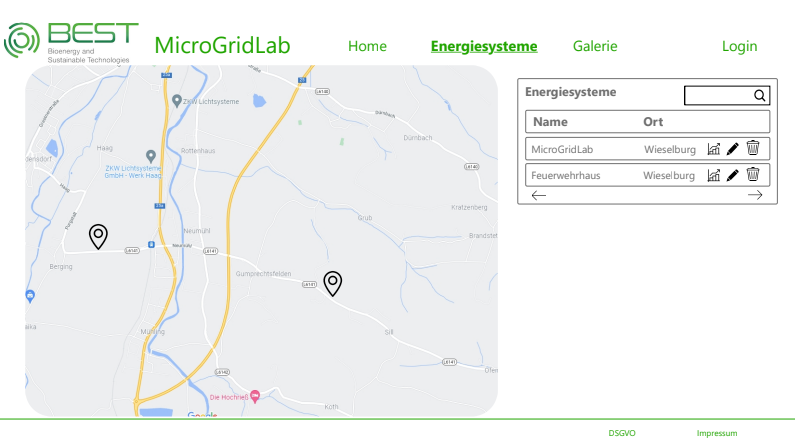
\includegraphics[height=7cm,width=12cm]{images/FinalerVorschlag}
	\caption{Finaler Design Vorschlag}
	\label{fig:Finaler Design Vorschlag}
\end{figure}
\newpage
Am Vorschlag in \ref{fig:Finaler Design Vorschlag}, wurde sich während der Entwicklung gerichtet. Aufgrund laufender Änderungswünsche des Auftraggebers variiert das finale Produktdesign jedoch stark vom finalen Vorschlag. Das finale Design ist im Kapitel \ref{sec: Front-End} einsehbar. 

\subsection{Definierte Farben}
Das Produktdesign basiert auf dem Front-End Framework Bootstrap. In Bootstrap werden alle Farben in der Datei “app.css” definiert. Hier ein textueller Ausschnitt, der vom Projektteam verwendeten Farben:
\\
\begin{figure}[h]
	\centering
	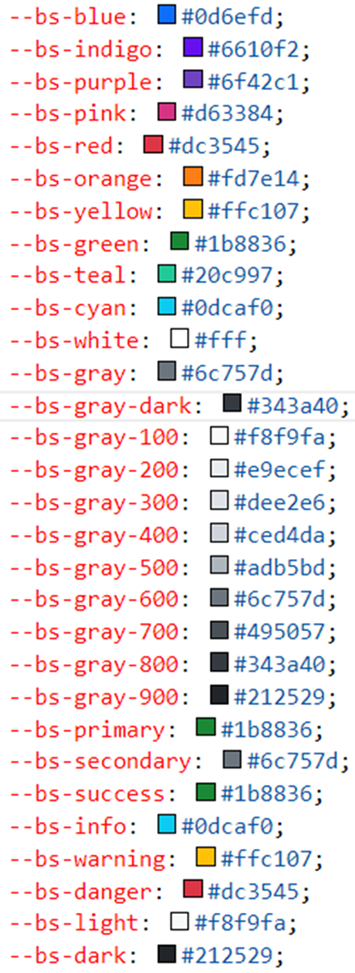
\includegraphics[height=15cm,width=4cm]{images/DefinierteFarben}
	\caption{Farben in Bootstrap}
	\label{fig: Farben in Bootstrap}
\end{figure}
\newpage
Auf Wunsch des Auftraggebers wurden jedoch einige Farben aus den CSS Dateien der bereits vorhanden Website extrahiert und bei diesem Produkt verwendet. Folgende Farben wurden extrahiert:
\\
\\
\begin{tabular}{|c|c|c|c|c|}
	\hline
	Hex & CMYK & RGB & HSV & HSL \\
	\hline
	\#1b8836 & 80\%, 0\%, 60\%, 47\% & 27, 136, 54 & 135, 80\%, 53\% & 135, 67\%, 32\%  \\
	\hline 
	\#f8f9fa & 1\%, 0\%, 0\%, 2\% & 247, 250, 250 & 80, 1\%, 98\% & 80, 23\%, 97\% \\
	\hline
	\#e84d3d & 0\%, 67\%, 74\%, 9\% & 232, 77, 61 & 6, 74\%, 91\% & 6, 79\%, 57\% \\
	\hline
	\#212529 & 20\%, 10\%, 0\%, 84\% & 33, 37, 41 & 210, 20\%, 16\% & 210, 11\%, 15\% \\
	\hline
	\#f1f1f1 & 19\%, 10\%, 0\%, 84\% & 241, 241, 241 & 210, 20\%, 16\% & 210, 11\%, 15\% \\
	\hline
	\#0d6efd & 95\%, 57\%, 0\%, 1\% & 13, 109, 252 & 216, 95\%, 99\% & 216, 98\%, 52\% \\
	\hline
	\#21a500 & 80\%, 0\%, 100\%, 35\% & 33, 166, 0 & 108, 100\%, 65\% & 108, 100\%, 33\% \\
	\hline
	
	
\end{tabular}

\subsection{Überschriften}
Überschriften werden bei diesem Produkt vorrangig verwendet, um anzuzeigen, über welches Thema der Fließtext, der sich meist direkt unter einer Überschrift befindet, handelt. Bei diesem Produkt wurden Überschriften der Gattung <h1>, <h2> und <h3> verwendet. Aus Design technischen Gründen, befindet sich jede Überschrift immer direkt in der Mitte der Website. Jede Überschrift, welche außerhalb eines Fließtextes steht, ist in der Farbe \#1b8836 eingefärbt und in der Schriftart Smooch Snans formatiert. Überschriften, welche sich in einem Fließtext befinden, werden in der Farbe \#212529 eingefärbt. Folgende Überschriften sind auf unserem Produkt vorhanden: 
\begin{itemize}
	\item Intelligente Strom- und Mikronetze
	\item Entwicklungsfelder und Anwendungsgebiete
	\item Forschungsprojekt Microgrid Lab
	\item Datenschutzerklärung
	\item DSGVO
	\item Impressum
\end{itemize}
\newpage
\begin{figure}[h]
	\centering
	\includegraphics[height=8cm,width=14cm]{images/UberschrieftenImFließtext}
	\caption{Überschriften im Fließtext}
	\label{fig: Überschriften im Fließtext}
\end{figure}
\begin{figure}[h]
	\centering
	
\includegraphics[height=8cm,width=14cm]{images/ImpressumUberschrift}
	\caption{Überschriften außerhalb des Fließtextes}
	\label{fig: Überschriften außerhalb des Fließtextes}
\end{figure}
\newpage

\subsection{Interaktionsfarben}
Interaktionsfarben werden verwendet, um eine Aktion zu kennzeichnen. Bei diesem  Produkt gibt es zwei verschiedene Interaktionsfarben. Die erste Farbe ist „\#21a500“ und die zweite „\#f1f1f1“. Die erste Farbe ist ersichtlich, wenn mit dem Mauszeiger über den Datatable gefahren wird. Und die zweite Farbe wird ersichtlich, wenn mit dem Mauszeiger auf das Drop-Down in der Galerie gefahren wird, um ein Energiesystem auszuwählen. Wenn dies geschieht, verfärben sich die einzelnen Auswahlelemente in die Farbe „\#f1f1f1“. 
\begin{figure}[h]
	\centering
	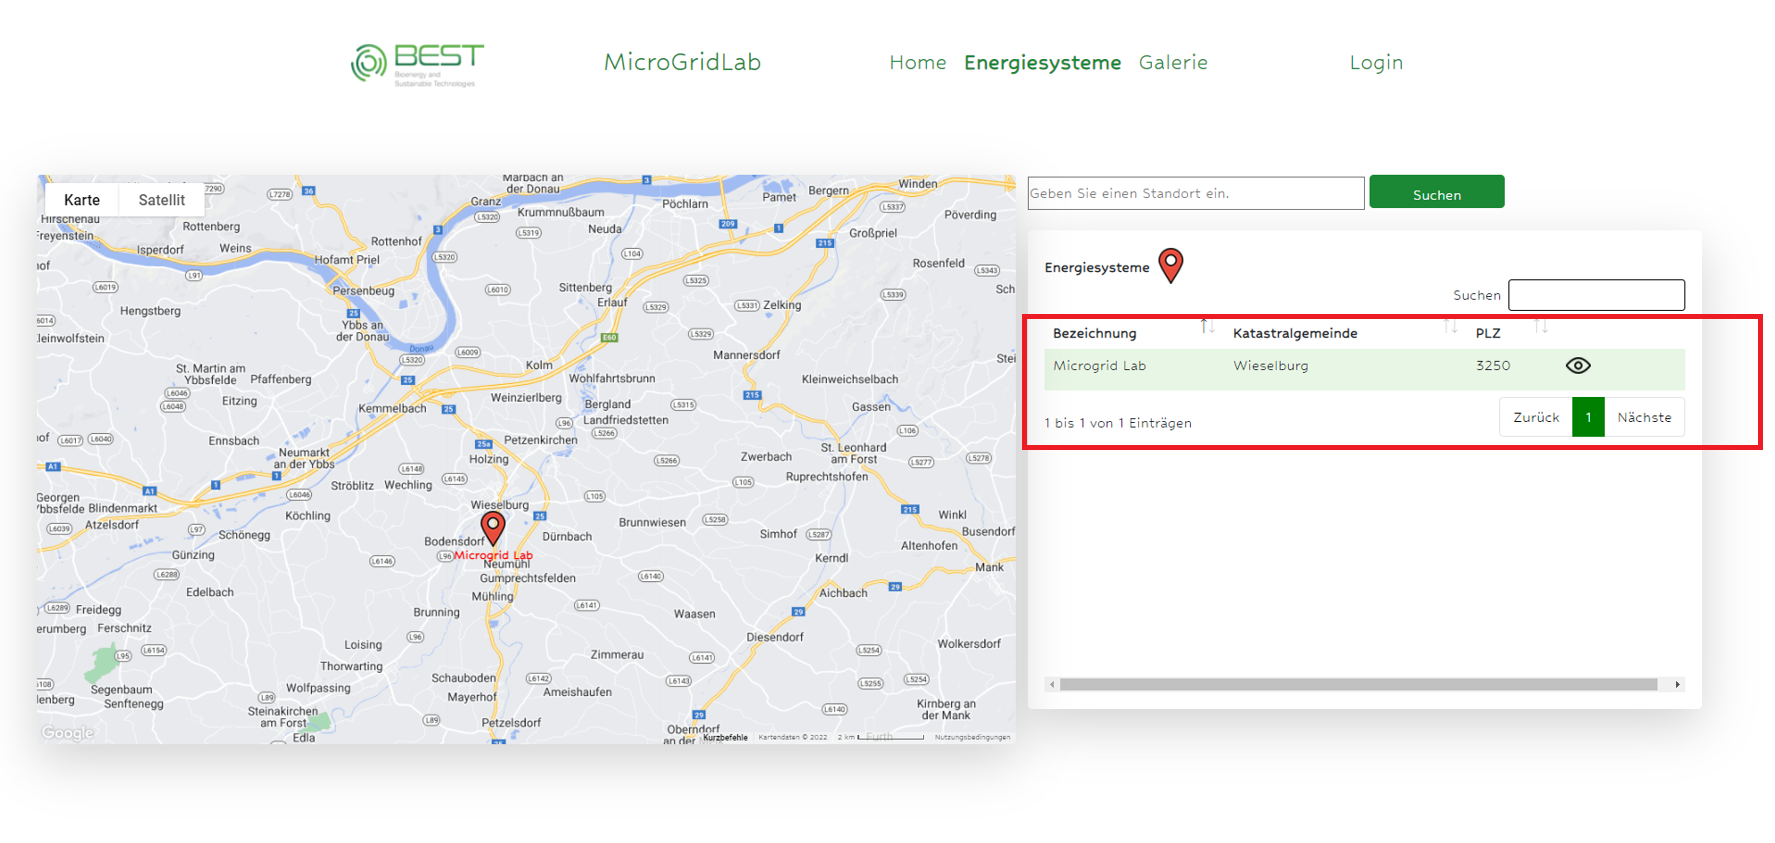
\includegraphics[height=8cm,width=15cm]{images/InteraktionDataTable}
	\caption{Interaktion mit dem Datatable}
	\label{fig: Interaktion mit dem Datatabel}
\end{figure}
\begin{figure}[h]
	\centering
	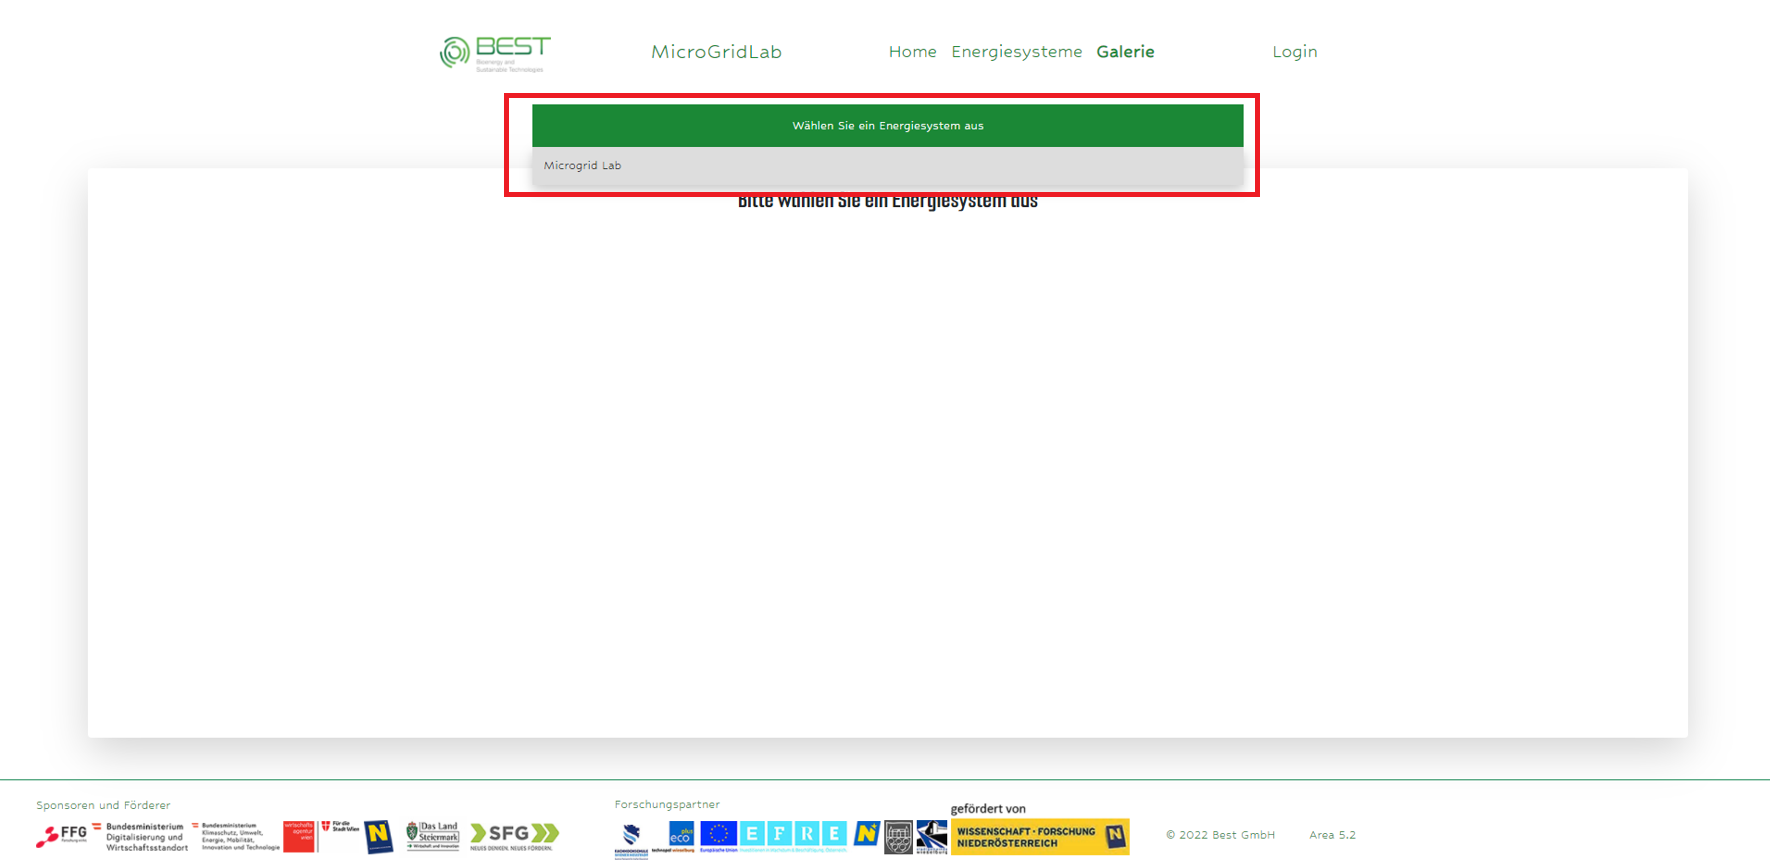
\includegraphics[height=8cm,width=15cm]{images/InteraktionDropDown}
	\caption{Interaktion mit dem Drop-Down in der Galerie}
	\label{fig: Interaktion mit dem Datatabel}
\end{figure}

\subsection{Schriftarten}
Unser Produkt verwendet die Schriftarten Smooch Sans und Hubballi. Diese Schriftarten sind von Google Fonts frei zur Verfügung und zur Verwendung gestellt. Hubballi wurde für jede Art von Fließtext verwendet. Smooch Snans wurde verwendet, um die Überschriften zu formatieren. Nachfolgend ein textueller Ausschnitt, um eine bessere Vorstellung über die Schriften zu bekommen:
\begin{figure}[h]
	\centering
	
\includegraphics[height=2cm,width=5cm]{images/HubaliBeispielstext}
	\caption{Beispielstext Hubballi}
	\label{fig: Beispielstext Hubballi}
\end{figure}
\begin{figure}[h]
	\centering
	
\includegraphics[height=2cm,width=5cm]{images/BeispielstextSmothSans}
	\caption{Beispielstext Smooch Snans}
	\label{fig: BeispielstextSmothSans}
\end{figure}
\subsection{Schriftgrade}
Die Schriftgrade variieren bei diesem Produkt nur bei der Anzeige der aktuellen Seite.
Die Überschriften Home, Energiesysteme und Galerie werden mithilfe des <b> Tags beim Besuchen der gleichnamigen Seite fett gemacht. Dadurch, dass die aktuelle Seite immer fett geschrieben wird, wird die Navigation durch das Produkt erleichtert.
\begin{figure}[h]
	\centering
	
\includegraphics[height=3cm,width=16cm]{images/Header}
	\caption{Header auf der Website}
	\label{fig: Header}
\end{figure}
\newpage
\subsection{Logo}
Beim Logo hat sich das Projektteam an den Wunsch des Auftraggebers gehalten und ein Logo, welches von Seitens des Auftraggebers zur Verfügung gestellt wurde, verwendet. Zwei Logos wurden zur Verfügung gestellt und gemeinsam wurde sich auf das Logo in Abbildung xy Logo 1 geeinigt. Das Projektteam rät jedoch dazu, bei Logos SVG Grafiken zu verwenden und nicht wie in diesem Fall eine JPG Grafik. Da dies jedoch für den Auftraggeber keine Relevanz hatte, wurde wie besprochen das Logo in Abbildung xy Logo 1 verwendet.
\\
\begin{figure}[h]
	\centering
	\includegraphics[height=3cm,width=14cm]{images/Logo1}
	\caption{Header auf der Website}
	\label{fig: Header}
\end{figure}
\\
\begin{figure}[h]
	\centering
	\includegraphics[height=3cm,width=14cm]{images/Logo2}
	\caption{Header auf der Website}
	\label{fig: Header}
\end{figure}


\subsection{Verwendete Icons und deren Bedeutungen} \label{sec:Verwendete Icons und deren Bedeutungen}
Bei diesem Produkt werden Icons verwendet, um Energiesysteme oder Energietechnologien auf der Map visuell darzustellen. Ein weiteres Einsatzgebiet der Icons sind Formulare oder Übersichten, wo sie Auskunft über die geforderten oder angezeigten Daten geben. Eine Liste mit allen Icons und deren Bedeutung ist hier zusammengefasst:


\begin{table}[]
	\caption{}
	\label{tab:my-table}
	\begin{tabular}{|l|l|}
		\hline
		
\includegraphics[height=1cm,width=1cm]{images/Icons/AzSpeicherES} & Zeigt die gesamte Verbraucher Energie                    \\ \hline
		
\includegraphics[height=1cm,width=1cm]{images/Icons/AzETES} & Zeigt die Anzahl der Energietechnologien                 \\ \hline
		
\includegraphics[height=1cm,width=1cm]{images/Icons/BildET}& Zeigt die Anzahl der Speicher in einem Energiesystem     \\ \hline
		\# & Zeigt die Anzahl der Verbraucher in einem Energiesystem  \\ \hline
		\# & Zeigt die  Gesamte Erzeuger und deren Leistung           \\ \hline
		\# & Zeigt die Katastralgemeinde in der sich ein Energiesystem befindet                     \\ \hline
		\# & Zeigt den Längengrad eines Energiesystems oder einer Energietechnologie                \\ \hline
		\# & Zeigt den Ort eines Energiesystems                       \\ \hline
		\# & Zeigt die Postleitzahl eines Energiesystems              \\ \hline
		\# & Zeigt den Typ der Energietechnologie                     \\ \hline
		\# & Zeigt die Beschreibung der Energietechnologie            \\ \hline
		\# & Zeigt die Bezeichnung des Energiesystems                 \\ \hline
		\# & Zeigt ein Bild der Energietechnologie                    \\ \hline
		\# & Zeigt den Breitengrad einer Energietechnologie oder eines Energiesystems               \\ \hline
		\# & Zeigt die gesamte  gesamte Energie einer Energietechnologie                            \\ \hline
		\# & Zeigt die gesamte Nennleistung eines Energiesystems      \\ \hline
		\# & Zeigt die gesamte Erzeuger Leistung eines Energiesystems \\ \hline
		\# & Zeigt die gesamte Erzeuger Energie in einem Energiesystem                              \\ \hline
		\# & Zeigt den aktuellen Netzbezug eines Energiesystems       \\ \hline
		\# & Symbolisiert ein Windkraftwerk                           \\ \hline
		\# & Symbolisiert eine Batterie                               \\ \hline
		\# & Symbolisiert einen Wärmespeicher                         \\ \hline
		\# & Symbolisiert ein Wasserstoffspeicher                     \\ \hline
		\# & Symbolisiert ein Wohnhaus                                \\ \hline
		\# & Symbolisiert einen Stromnetzbezug                        \\ \hline
		\# & Symbolisiert eine Solartherme                            \\ \hline
		\# & Symbolisiert einen saisonalen Wärmespeicher              \\ \hline
		\# & Symbolisiert eine Pv-Anlage                              \\ \hline
		\# & Symbolisiert ein E-Tankstelle                            \\ \hline
		\# & Symbolisiert eine Gemeinde                               \\ \hline
		\# & Symbolisiert ein Haus                                    \\ \hline
		\# & Symbolisiert eine Raffinerie                             \\ \hline
		\# & Symbolisiert eine Wärmepumpe                             \\ \hline
		\# & Symbolisiert eine Ab oder Absorptionskältemaschine       \\ \hline
		\# & Symbolisiert eine Kompressionskältemaschine              \\ \hline
		\# & Symbolisiert einen Kältespeicher                         \\ \hline
		\# & Symbolisiert eine Industrie                              \\ \hline
		\# & Symbolisiert einen Gebäude Kältebedarfszähler            \\ \hline
		\# & Symbolisiert einen Elektrolyseur                         \\ \hline
		\# & Symbolisiert ein Biomasseheizkraftwerk                   \\ \hline
		\# & Symbolisiert einen Biomassekessel                        \\ \hline
		\# & Symbolisiert ein Elektroauto                             \\ \hline
		\# & Symbolisiert eine Brennstoffzelle                        \\ \hline
		\# & Symbolisiert ein Energiesystem auf der Karte             \\ \hline
		\# & Symbolisiert ein Energiesystem auf der Karte, sobald dieses ausgewählt wurde           \\ \hline
		\# & Symbolisiert eine Energietechnologie auf der Karte       \\ \hline
		\# & Statistiken eines Energiesystems bei klick auf Auge Icon \\ \hline
		\# & Löschen eines Energiesystems oder einer Energietechnologie bei Klick auf den Mülleimer \\ \hline
		\# & Grafana Statistiken bei Klick auf das Icon               \\ \hline
		\# & Bearbeiten einer Energietechnologie oder eines Energiesystems                          \\ \hline
	\end{tabular}
\end{table}
\newpage
\subsection{Map Icons}
Das Produkt verwendet die vom Auftraggeber bereitgestellte Icons, um Energietechnologien oder Energiesystem auf der Karte visuelle darzustellen. Die Icons auf der Map sehen folgendermaßen aus:
\begin{figure}[h]
	\centering
	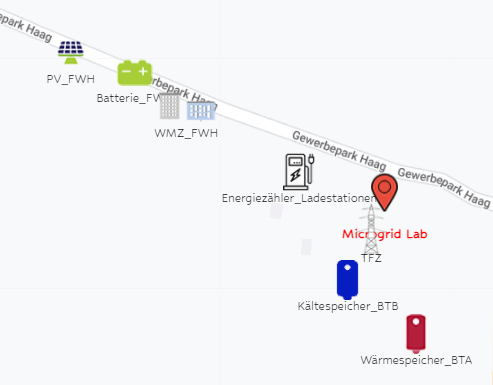
\includegraphics[height=6cm,width=10cm]{images/MapIcons}
	\caption{Icons auf der Map}
	\label{fig: Icons auf der Map}
\end{figure}
\\
Um Energiesysteme oder Energietechnologien zu verzeichnen, werden folgende Icons verwendet: 
\begin{figure}[h]
	\centering
	
\includegraphics[height=1cm,width=1cm]{images/Icons/esrot}
	\caption{Icon markiert ein Energiesystem}
	\label{fig: EnergiesystemIcon}
\end{figure}
\begin{figure}[h]
	\centering
	
\includegraphics[height=1cm,width=1cm]{images/Icons/etrot}
	\caption{Icon markiert eine Energietechnologie}
	\label{fig: EnergietechnologieIcon}
\end{figure}



\subsection{Icons in Formularen}
Alle weiteren verwendeten Icons wurden von flaticons.com implementiert. Diese Icons werden dazu genutzt, um in Formularen anzuzeigen, welche Art von Wert verlangt wird. Des Weiteren werden diese Icons in Übersichten verwendet, um dem Benutzer anzuzeigen, um welchen Wert es sich handelt. Um diese Icons jedoch verwenden zu dürfen, mussten alle Autoren in der Datenschutzseite verlinkt werden. Hier ein Beispiel, wie diese Anwendungsfälle auf der Website aussehen:
\begin{figure}[h]
	\centering
	\includegraphics[height=10cm,width=5cm]{images/IconsInÜbersichten}
	\caption{Icon in Übersichten}
	\label{fig: Icons in Übersichten}
\end{figure}
\newpage
\begin{figure}[h]
	\centering
	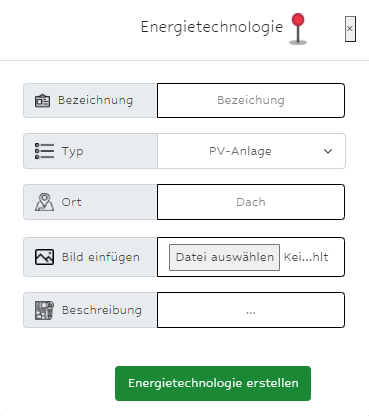
\includegraphics[height=6cm,width=5cm]{images/IconsInFormularen}
	\caption{Icon in Formularen}
	\label{fig: Icons in Formularen}
\end{figure}
\newpage
Aus Lizenztechnischen Gründen wurde jeder Autor eines Icons auf unserer Seite im Datenschutz verlinkt. Dies sieht folgendermaßen aus:
\begin{figure}[h]
	\centering
	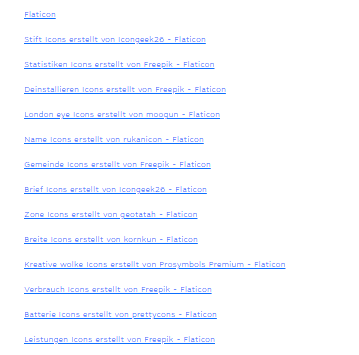
\includegraphics[height=10cm,width=7cm]{images/IconAutorVerlinkungen}
	\caption{Autoren Verlinkungen}
	\label{fig: Autoren Verlinkungen}
\end{figure}

\newpage
\subsection{Icons im DataTable}
Folgende Icons werden  verwendet, um Energiesystem oder Energietechnologien zu bearbeiten, zu löschen oder auf deren Grafana Statistiken zuzugreifen.
\begin{table}[h]
	\caption{}
	\label{tab:my-table}
	\begin{tabular}{|l|l|}
		\hline
		Icon & Funktion                                                                                     \\ \hline
			
\includegraphics[height=1cm,width=1cm]{images/Icons/statistik}& Mit einem Klick auf dieses Icon öffnet sich ein Pop-up,\\& auf welchem die dazugehörigen  Grafana Statistiken präsentiert werden       \\ \hline
			
\includegraphics[height=1cm,width=1cm]{images/Icons/delete}  & Mit einem Klick auf dieses Icon wird das ausgewählte Energiesystem gelöscht                  \\ \hline
			
\includegraphics[height=1cm,width=1.5cm]{images/Icons/auge} & Mit einem Klick auf dieses Icon werden erweiterte Infos zu dem ausgewählten System angezeigt \\ \hline
			
\includegraphics[height=1cm,width=1cm]{images/Icons/stift} & Mit einem Klick auf dieses Icon öffnet sich eine Bearbeitungsmöglichkeit,\\& auf welcher man die Eigenschaften des Systems ändern kann \\ \hline
	\end{tabular}
\end{table}

Auf der Website werden diese Icons im Datatable hinter einer Energietechnologie oder einem Energiesystem eingeblendet. Dies sieht folgendermaßen aus:
\begin{figure}[h]
	\centering
	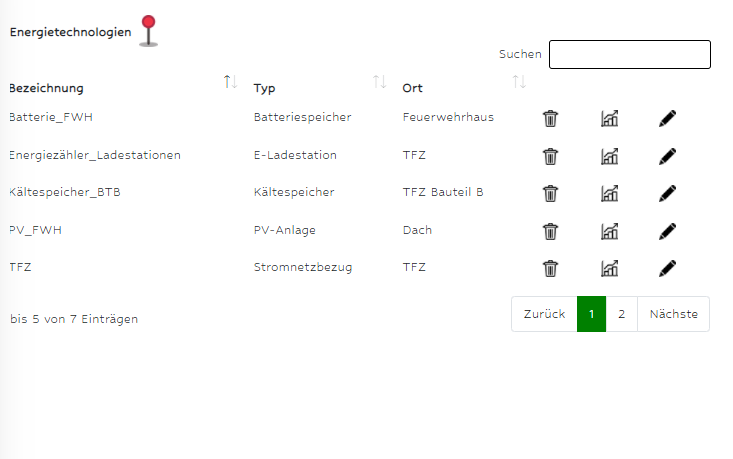
\includegraphics[height=10cm,width=15cm]{images/IconsImDatatable}
	\caption{Icons im Datatable}
	\label{fig: Icons im Datatable}
\end{figure}


\subsection{Buttons}
Buttons werden bei diesem Produkt ausschließlich genutzt, um Formulare abzusenden. Buttons befinden sich immer mittig unter einem Formular und  haben die Hintergrundfarbe \#1b8836. Folgende Buttons wurden verwendet: 

\subsection{Tabelle mit generellen Informationen über einzelne HTML Elemente}
Hier ist wichtig zu definieren für was welches HTML Element verwendet wurde. <h1>,  <h2> und <h3> wurden verwendet um Überschriften zu definieren. In einem <p> Element befindet sich immer ein Fließtext. Mit dem <a> Element werden Links definiert. Bei diesem Produkt wurden im Header die Navigationsmöglichkeiten mit diesem Element versehen. 
\begin{table}[h]
	\caption{}
	\label{tab:genrelle Infos}
	\begin{tabular}{|l|l|l|l|l|}
		\hline
		HTML Element                & Schriftart  & Größe  & Farbe              & Style class oder id   \\ \hline
		\textless{}h1\textgreater{} & Smooch Sans & 2em & \#1b8836  \#212529 & \begin{tabular}[c]{@{}l@{}}DsgvoUberschrift\\ ImpressumUberschrieft\end{tabular} \\ \hline
		\textless{}h2\textgreater{} & Smooch Sans & 1.5em  & \#1b8836  \#212529 & NavUberschrift        \\ \hline
		\textless{}h3\textgreater{} & Smooch Sans & 1.17em & \#1b8836  \#212529 & FliesstextUberschrift \\ \hline
		\textless{}p\textgreater{}  & Hubballi    & -      & \#000000           & text-primary          \\ \hline
		\textless{}a\textgreater{}  & Hubballi    & -      & \#1b8836           & dropdown-item         \\ \hline
	\end{tabular}
\end{table}


\subsection{Datenformate}
Auf dem Produkt befindet sich eine Diashow, die Bilder des Projektes Micro Grid Lab der Best GmbH präsentiert. Alle diese Bilder haben das Dateiformat JPG. Eines der präsentierten Bilder ist im Dateiformat PNG. Alle verwendeten Icons sind als PNG auf dem Produkt eingebunden. Die Fotos der Sponsoren aus dem Footer sind gemischt im PNG und im JPG Format. Das Logo, wie bereits im Kapitel 2.6.5.6 erwähnt, ist im Format JPG. Hier rät das Projektteam jedoch dazu, eine Vektorgrafik mit dem Dateiformat SVG zu verwenden.


\section{Weboberfläche}
Im Abschnitt Weboberfläche wird speziell auf das Front-End sowie das Back-End des Produktes eingegangen. Bei dem Punkt Back-End vor allem auf die Funktionen, die für die Benutzer-Interaktionen zuständig sind, und bei dem Punkt Front-End auf das Layout sowie das Design der Weboberfläche.


\subsection{Backend}
In diesem Abschnitt wird genauer auf den Ablauf des Codes im Back-End, der für die Funktionen auf der Weboberfläche zuständig ist, eingegangen. 
Für jedes Energiesystem oder jede Energietechnologie stehen die Funktionen Erstellen, Bearbeiten und Löschen zur Verfügung. In den folgenden Abschnitten wird genauer auf diese Funktionen eingegangen.


\subsubsection{Energiesystem Erstellen}
Für das Erstellen eines Energiesystems ist ein Mausklick auf der Karte notwendig. Daraufhin öffnet sich ein Pop-up Fenster, um die Kerndaten des Energiesystems einzugeben.
Das Pop-up zum Erstellen eines Energiesystems ist in der Abbildung x.y ersichtlich.
Beim Erstellen eines Energiesystems werden folgende Attribute in der Datenbank erfasst:
Eingabe des Benutzers:
\begin{itemize}
	\item Bezeichnung 
	\item Katastralgemeinde
	\item Postleitzahl
\end{itemize}

Automatisch ausgefüllte Attribute, welche nicht im Pop-up dargestellt werden:
\begin{itemize}
	\item Längengrad 
	\item Breitengrad
	\item User\_ID
\end{itemize}


\begin{figure}[h]
	\centering
	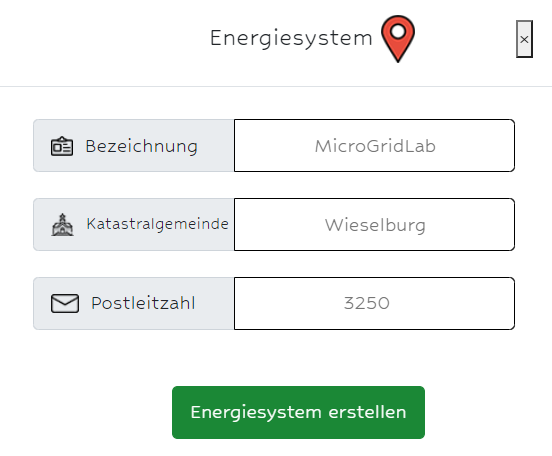
\includegraphics[height=8cm,width=9cm]{images/ESerstellenPop}
	\caption{Energiesystem Erstellen Pop-up}
	\label{fig:CSS_System}
\end{figure}
\newpage
Die Attribute Längengrad und Breitengrad werden automatisch mithilfe des Mausklicks auf der Karte mit den entsprechenden Koordinaten beim Erstellen des Energiesystems befüllt. Das Attribut User\_ID wird automatisch mit der ID des gerade angemeldeten Benutzers ausgefüllt, um das Energiesystem einem Benutzer zuteilen zu können.
Nachdem der Benutzer alle Daten eingegeben hat, werden diese Daten an den Controller übermittelt, wo anschließend das Energiesystem erstellt und in der Datenbank erfasst wird. Als nächstes werden die gespeicherten Informationen wieder zurück an die Weboberfläche übergeben, um die Energiesysteme-Marker auf der Karte zu platzieren sowie den Inhalt der Liste aller vorhandenen Energiesysteme zu aktualisieren. Die folgende Abbildung zeigt den Ablauf, um ein Energiesystem zu erstellen:

\begin{figure}[h]
	\centering
	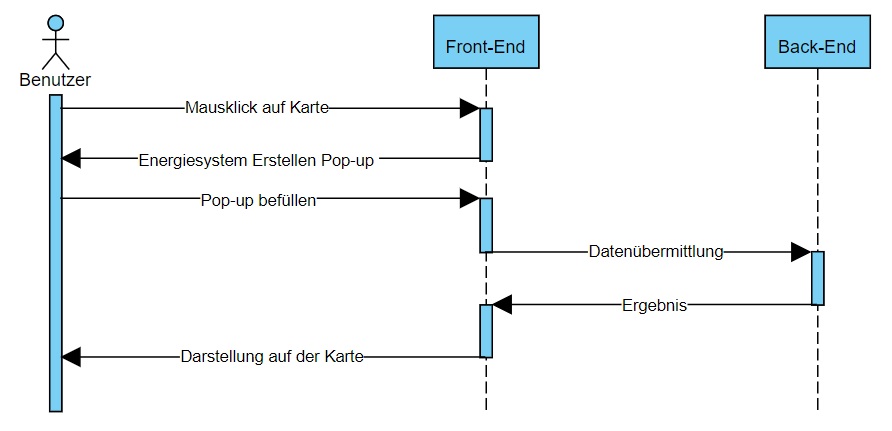
\includegraphics[height=7cm,width=14cm]{images/ESerstellen}
	\caption{Energiesystem Erstellen}
	\label{fig:CSS_System}
\end{figure}





\subsubsection{Energiesystem Bearbeiten}
Mit dem Stift-Icon beim Energiesystem in der Liste ist es möglich, die Kerndaten eines Energiesystems zu bearbeiten. Die zu bearbeitenden Daten, welche einen weißen Hintergrund  aufweisen, lauten auf „Bezeichnung“, „Katastralgemeinde“ und „Postleitzahl“. Die Koordinaten sowie die User\_ID des Energiesystems bleiben konstant und sind nicht änderbar und nicht im Pop-up ersichtlich.
Folgende weitere Attribute werden bei jedem Energiesystem automatisch berechnet, angezeigt und sind nicht bearbeitbar, sondern dienen nur als weitere Information über das ausgewählte Energiesystem. Das Pop-up zum Bearbeiten eines Energiesystems ist in der Abbildung x.y ersichtlich.
\begin{figure}[h]
	\centering
	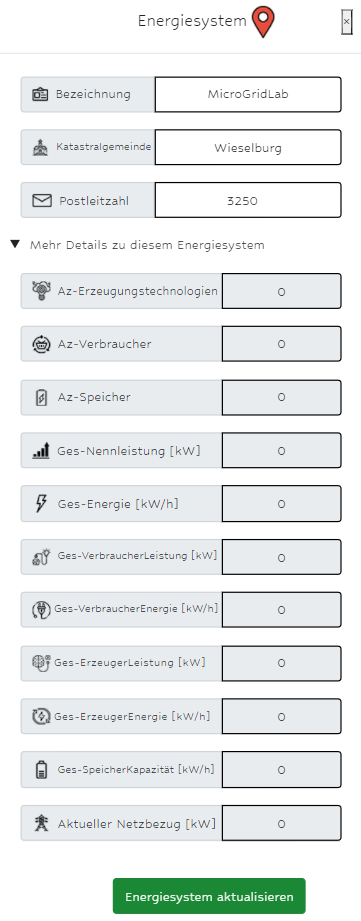
\includegraphics[height=16cm,width=6cm]{images/ESbearbeitenPop}
	\caption{Energiesystem Bearbeiten Pop-up}
	\label{fig:CSS_System}
\end{figure}
\newpage
\begin{itemize}
	\item Anzahl-Erzeugungstechnologien  
	\item Anzahl-Verbraucher
	\item Anzahl-Speicher
	\item Ges-Nennleistung [kW]
	\item Ges-Energie [kW/h]
	\item Ges-Verbraucher-Leistung [kW]
	\item Ges-Verbraucher-Energie [kW/h]
	\item Ges-Erzeuger-Leistung [kW]
	\item Ges-Erzeuger-Energie [kW/h]
	\item Ges-Speicher-Kapazität [kW/h]
	\item Aktueller Netzbezug [kW]
\end{itemize}

Für genauere Informationen zu den einzelnen Attributen siehe Kapitel  \ref{sec:Verwendete Icons und deren Bedeutungen}
Mit dem Button „Mehr Details zu diesem Energiesystem“ ist es möglich, die weiteren Daten des Energiesystems ein- und auszuklappen. 
Nachdem der Benutzer die Attribute des Energiesystems bearbeitet hat, werden diese mithilfe des Controllers in der Datenbank aktualisiert. Anschließend werden die neuen Daten der Weboberfläche übergeben, um auf der Karte sowie in der Liste den aktuellen Stand der Energiesysteme darstellen zu können. In der Abbildung x.y ist der Ablauf „Energiesystem bearbeiten“ dargestellt:
\newline
\begin{figure}[h]
	\centering
	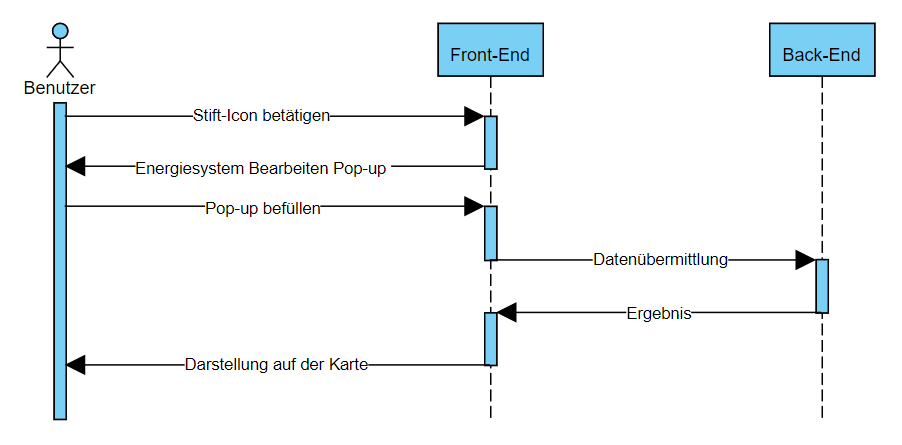
\includegraphics[height=7cm,width=14cm]{images/ESbearbeiten}
	\caption{Energiesystem Bearbeiten}
	\label{fig:CSS_System}
\end{figure}


\subsubsection{Energiesystem Löschen}
Um ein Energiesystem zu löschen, benötigt man das Mülleimer-Icon, welches sich neben jedem Energiesystem in der Liste befindet, sofern der angemeldete Benutzer die erforderliche Berechtigung dazu hat. 
Nachdem dieses Icon betätigt wurde, wird die Information, dass ein Energiesystem gelöscht wurde, an den Controller übermittelt. Dieser löscht anschließend mithilfe der ID des ausgewählten Energiesystems dieses aus der Datenbank und übergibt alle anderen Energiesysteme zurück auf die Weboberfläche, um die vorhandenen Energiesysteme auf der Karte zu platzieren sowie in der Liste anzuzeigen. Der Ablauf, um ein Energiesystem zu löschen, wird in folgendem Diagramm präsentiert:
\newline
\begin{figure}[h]
	\centering
	\includegraphics[height=7cm,width=14cm]{images/ESlöschen}
	\caption{Energiesystem Löschen}
	\label{fig:CSS_System}
\end{figure}

\newpage
\subsubsection{Energietechnologie Erstellen}
Für das Erstellen einer Energietechnologie ist das Auswählen eines Energiesystems mit einem Doppelklick notwendig. Anschließend verwandelt sich der Cursor in das Energietechnologie-Icon, welches darauf hindeutet, dass jetzt das Hinzufügen einer Energietechnologie mittels eines Klicks auf der gewünschten Position auf der Karte möglich ist. Nach dem Klick auf der Karte öffnet sich ein Pop-up-Fenster, um die Kerndaten der Energietechnologie einzugeben. Dieses Pop-up ist in der Abbildung x.y ersichtlich. 
\begin{figure}[h]
	\centering
	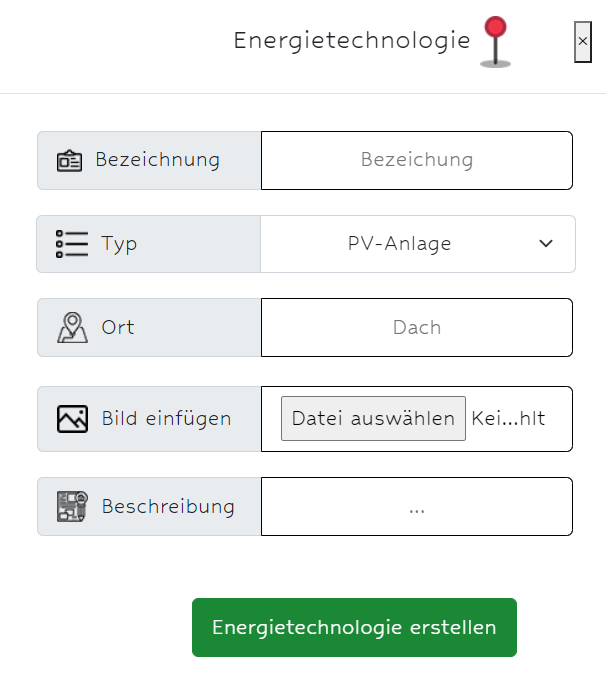
\includegraphics[height=11cm,width=8cm]{images/ETerstellenPop}
	\caption{Energietechnologie Erstellen Pop-up}
	\label{fig:CSS_System}
\end{figure}

\newpage
Eingabe des Benutzers:
\begin{itemize}
	\item Bezeichnung 
	\item Typ
	\item Ort
	\item Bild einfügen
	\item Beschreibung
\end{itemize}

Automatisch ausgefüllt und nicht im Pop-up dargestellt:
\begin{itemize}
	\item Längengrad 
	\item Breitengrad
	\item Ensys\_ID
	\item User\_ID
\end{itemize}

Nachdem der Benutzer die Daten im Pop-up ausgefüllt hat, werden diese Informationen über den Controller in der Datenbank erfasst. Anschließend werden die Energietechnologie-Daten an die Weboberfläche übermittelt, um die Energietechnologien auf der Karte darzustellen sowie in der Liste anzuzeigen. Der Ablauf, um eine Energietechnologie zu erstellen, wird in der Abbildung x.y dargestellt:
 \begin{figure}[h]
 	\centering
 	\includegraphics[height=7cm,width=14cm]{images/ETerstellen}
 	\caption{Energietechnologie Erstellen}
 	\label{fig:CSS_System}
 \end{figure}


\subsubsection{Energietechnologie Bearbeiten}
Um eine Energietechnologie zu bearbeiten, muss zuerst ein Energiesystem mit einem Doppelklick ausgewählt werden. Anschließend befinden sich rechts in der Liste alle dazugehörigen Energietechnologien, welche man mit dem Stift-Icon bearbeiten kann. Nach dem Betätigen des Stift-Icons öffnet sich ein Pop-up-Fenster, um die Attribute zu bearbeiten. Dieses Pop-up-Fenster ist in der Abbildung x.y ersichtlich.
\newline
\begin{figure}[h]
	\centering
	\includegraphics[height=11cm,width=8cm]{images/ETbearbeitenPop}
	\caption{Energietechnologie Bearbeiten}
	\label{fig:CSS_System}
\end{figure}


Dabei sind die Attribute „Bezeichnung“, „Ort“, „Bild“ und „Beschreibung“ bearbeitbar. Um dem Benutzer dies deutlich zu machen, weisen diese Attribute einen weißen Hintergrund auf. 
Die Attribute „Typ“, „Längengrad“, „Breitengrad“, „Ensys\_ID“ sowie „User\_ID“ sind nicht bearbeitbar.
Nachdem der Benutzer die Daten bearbeitet hat, werden diese über den Controller in die Datenbank geschrieben. Anschließend werden die Energietechnologie-Daten an die Weboberfläche übergeben, um die Marker auf der Karte zu platzieren sowie den Inhalt der Liste zu aktualisieren. 
\newpage
Das nachfolgende Diagramm beschreibt den Ablauf für das Bearbeiten einer Energietechnologie:
\newline
\begin{figure}[h]
	\centering
	\includegraphics[height=7cm,width=14cm]{images/ETbearbeiten}
	\caption{Energietechnologie Löschen}
	\label{fig:CSS_System}
\end{figure}

\newpage
\subsubsection{Energietechnologie Löschen}
Um eine Energietechnologie zu löschen, benötigt man das Mülleimer-Icon, welches sich in der Liste neben den Energietechnologien befindet, sofern ein Energiesystem von dem Benutzer ausgewählt wurde.
Sobald der Benutzer dieses Icon betätigt, wird mithilfe der ID der ausgewählten Energietechnologie dem Controller mitgeteilt, dass diese Energietechnologie gelöscht werden soll. Daraufhin löscht der Controller diese Energietechnologie aus der Datenbank und übergibt anschließend alle anderen vorhandenen Energietechnologie-Daten an die Weboberfläche, um dort die Marker zu platzieren sowie den Inhalt der Liste zu aktualisieren. Das nachfolgende Diagramm beschreibt den Ablauf für das Löschen einer Energietechnologie:
\begin{figure}[h]
	\centering
	\includegraphics[height=7cm,width=14cm]{images/ETlöschen}
	\caption{Energietechnologie Löschen}
	\label{fig:CSS_System}
\end{figure}


\newpage
\subsubsection{Benutzerverwaltung}
Je nach Benutzerrolle des aktuell angemeldeten Benutzers stehen dem Benutzer unterschiedliche Funktionen auf der Weboberfläche zur Verfügung.  
Folgende drei Benutzer stehen zur Verfügung:
\begin{itemize}
	\item Administrator 
	\item Mitarbeiter
	\item Öffentlicher Benutzer
\end{itemize}
Wie eine generelle Überprüfung des Benutzers in Laravel umgesetzt werden kann, ist unter der Quelle x.y ersichtlich. Folgende Überprüfung wurde selbst vom Projektteam entwickelt und ist somit nicht unter der genannten Quelle auffindbar.\newline \newline
Mit folgender Überprüfung wird kontrolliert, ob der gerade angemeldete Benutzer das Energiesystem oder die Energietechnologie selbst erstellt hat oder ob er die Rolle des Administrators aufweisen kann. Falls der Benutzer das Energiesystem oder die Energietechnologie selbst erstellt hat, ist der erste Teil der Überprüfung erfüllt und der Benutzer hat die Verwaltungsfunktionen zur Verfügung. Falls der Benutzer das Energiesystem oder die Energietechnologie nicht selbst erstellt hat, wird die zweite Überprüfung durchgeführt, welche überprüft, ob der Benutzer die Rolle des Administrators aufweisen kann. Falls er diese Rolle besitzt, hat er die Verwaltungsfunktionen zur Verfügung, andernfalls nicht.


\begin{lstlisting}[
	caption={Funktion Blade.php Zeile 1-2},
	label=Code,
	language=octave,
	numbers=left,
	firstnumber=100,
	numberfirstline=false,
	backgroundcolor=\color{mygray},
	basicstyle=\footnotesize=15,
	keywordstyle=\color{blue}
	]
	
@if ($userID->id == $d->users_idusers || $userID->role == 'Admin')

	
\end{lstlisting}





\subsubsection{Adresssuche}
Mithilfe des Adresssuchfeldes ist es möglich, einen Standort einzugeben, um anschließend auf der Karte zu diesem zu gelangen. Dadurch ist das Auffinden von bestimmten Orten auf der Karte problemlos möglich. Dabei wird die eingegebene Adresse in geografische Koordinaten umgewandelt, zu welchen man anschließend navigiert wird. In der folgenden Abbildung ist das Adresssuchfeld ersichtlich.
\begin{figure}[h]
	\centering
	\includegraphics[height=2cm,width=15cm]{images/Adresssuchfeld}
	\caption{Adresssuchfeld}
	\label{fig:Adresssuchfeld}
\end{figure}

\newpage
Folgende Schreibweisen sind in der Suche möglich:
\begin{itemize}
	\item Stadt 
	\item Land
	\item Straße 
	\item Postleitzahl 
\end{itemize}


\textbf{Automatische Vervollständigung} \\
Um die Suche nach der richtigen Adresse zu vereinfachen, wird die Eingabe des Benutzers mit einer Auto-Complete-Funktion unterstützt. Diese Funktion bietet mögliche Ziel-Adressen anhand der bisher eingegebenen Daten an, welche vom Benutzer ausgewählt werden können. Ein Beispiel dieser Funktion ist in der Abbildung x.y dargestellt. 
\begin{figure}[h]
	\centering
	\includegraphics[height=7cm,width=15cm]{images/Vorschläge}
	\caption{Automatische Vervollständigung}
	\label{fig:Automatische Vervollständigung}
\end{figure}
\\

\newpage
\textbf{Adresssuche durchführen} \\
Die Adresssuche kann auf zwei verschiedene Arten durchgeführt werden.
Die erste Variante ist das Benutzen des dazugehörigen Buttons mit der Beschriftung „Suchen“. Die zweite Variante ist das Betätigen der Enter-Taste auf der Tastatur. Beide Varianten führen zu dem gleichen Ergebnis, und zwar, dass die Adresssuche durchgeführt wird.
Sobald die Adresssuche durchgeführt wird, werden für die eingegebene Adresse die dazugehörigen Koordinaten berechnet. Sobald diese berechnet wurden, werden diese an die Karte übergeben, damit der Mittelpunkt der Karte auf diese Koordinaten gesetzt wird. Anschließend gelangt der Benutzer zu seiner eingegebenen Adresse auf der Karte und kann seine Interaktionen fortsetzen. Das folgende Diagramm beschreibt die Durchführung der Adresssuche:
\begin{figure}[h]
	\centering
	\includegraphics[height=7cm,width=14cm]{images/Adresssuche}
	\caption{Adresssuche}
	\label{fig:Adresssuche }
\end{figure}
\\

\newpage
\subsection{Front-End} \label{sec: Front-End}
Das Projektteam hat sich bei der Front-End Gestaltung an die Vorgabe des Auftraggebers gehalten und sich an der bereits vorhanden Website der Best Gmbh orientiert. Das Produkt wurde dann mithilfe der Laravel Layout Funktion in Header Footer und Content unterteilt. Nähere Informationen dazu sind im Kapitel 3.5.4 vermerkt. Generell ist das Produkt gegliedert in folgende Unterseiten: 
\begin{itemize}
	\item Home 
	\item Energiesysteme
	\item Galerie 
	\item Impressum 
	\item Datenschutz
	\item Registrierungsseite
\end{itemize}
Auf die oben aufgezählten Unterseiten wird in den nachfolgenden Kapiteln genauer eingegangen.

\subsubsection{Home}
Die Home Seite ist die erste Seite, die ein Benutzer zu Gesicht bekommt, wenn er das Produkt aufruft. Die Seite besteht aus einer Diashow, die Bilder des Micro Grid Lab Projekts der Best GmbH zeigt. Unter dieser befindet sich ein Textbereich, auf welchem sich das Projekt “Micro Grid Lab” kurz vorgestellt wird. Hier ein Bild der besagten Seite:
\begin{figure}[h]
	\centering
	\includegraphics[height=7cm,width=14cm]{images/HomeSeite1}
	\caption{oberer Teil der Home Seite}
	\label{fig:HomeSeite1}
\end{figure}
\begin{figure}[h]
	\centering
	\includegraphics[height=7cm,width=14cm]{images/HomeSeite2}
	\caption{unterer Teil der Home Seite}
	\label{fig:HomeSeite1}
\end{figure}

\subsubsection{Energiesysteme}
Die Energiesysteme Seite ist die Seite, wo die Hauptfunktion des Produkts verwendet werden kann. Auf dieser wird die Verwaltung der Energiesysteme und Energietechnologien mithilfe einer Map visuell dargestellt. Diese Seite besteht aus einer Google Maps Karte, welche sich auf der linken Seite der Website befindet. Ebenso einem Datatable auf der rechten Hälfte der Website. Hier ein Bild der eben beschriebenen Seite:
\begin{figure}[h]
	\centering
	\includegraphics[height=6cm,width=14cm]{images/EnergiesystemSeite}
	\caption{die Energiesystem Seite}
	\label{fig:Energiesystem Seite}
\end{figure}
\newpage

\subsubsection{Galerie}
Das Produkt bietet auch die Möglichkeit, zu jeder Energietechnologie ein dementsprechendes Bild zu speichern. Dieses Bild wird dann in der Bildergalerie angezeigt. Durch einen Dropdown, welches sich oben in der Mitte der Seite befindet, kann ein Energiesystem auswählt werden. Von diesem ausgewählten Energiesystem werden dann alle dazugehörigen Energietechnologien mit dem entsprechendem Bild angezeigt. Die Galerie sieht folgendermaßen aus:
\begin{figure}[h]
	\centering
	\includegraphics[height=6cm,width=14cm]{images/GalerieSeite}
	\caption{die Galerie}
	\label{fig:Galerie}
\end{figure}


\subsubsection{Impressum}
Auf der Impressumsseite, welche durch den Footer erreichbar ist, ist das Impressum der Website einsehbar. Die Seite hat eine Überschrift  “Impressum” und darunter befindet sich ein Textbereich  mit dem dazugehörigen Impressum. Am Ende des Impressums befindet sich noch ein Link, welcher auf die Homepage der Best GmbH weiterleitet. Hier ist ein Foto der Impressum Seite:

\begin{figure}[h]
	\centering
	\includegraphics[height=6cm,width=14cm]{images/ImpressumSeite}
	\caption{das Impressum}
	\label{fig:Impressum}
\end{figure}
\newpage
\subsubsection{Datenschutz}
Wie auch die Impressumsseite ist die Datenschutzseite durch den Footer erreichbar. Diese ist gleich aufgebaut wie die Impressumsseite. Auch hier gibt es wieder mittig eine Überschrift “Datenschutz”, unter welcher wieder ein Textbereich vorhanden ist. In diesem Textbereich  ist die Datenschutzgrundverordnung des Produkts einsehbar.  Hier ein Foto der Datenschutzseite:
\begin{figure}[h]
	\centering
	\includegraphics[height=6cm,width=14cm]{images/DSGVOSeite}
	\caption{die Datenschutz Seite}
	\label{fig:DSGVO}
\end{figure}
\subsubsection{Registrierungsseite}
Die Registrierungsseite kann nur von einem Administrator erreicht werden. Auf dieser Seite ist es möglich, neue Benutzer zu registrieren und bereits vorhandene Benutzer zu löschen. Genauere Informationen zu dieser Seite sind im Kapitel 3.5.3 nachlesbar. Hier ein Foto der Registerseite:
\begin{figure}[h]
	\centering
	\includegraphics[height=7cm,width=14cm]{images/RegisterSeite}
	\caption{die Registrierungsseite }
	\label{fig:RegisterSeite}
\end{figure}
\newpage


\subsection{Login}
Möchte sich ein Benutzer beim Produkt anmelden, kann er dies beim Login Feld, welches in  Abbildung xy Login Feld ersichtlich ist. Dort meldet er sich mit einer E-Mail-Adresse und einem Passwort an, welche vorher auf der Registrierungsseite angelegt wurde. Nach Eingabe  der Daten ,wird überprüft ob die Daten in der Datenbank vorhanden sind und das Passwort richtig eingegeben wurde. Das Login feld sieht folgendermaßen aus :

\begin{figure}[h]
	\centering
	\includegraphics[height=5cm,width=7cm]{images/LoginFeld}
	\caption{das Login Formular}
	\label{fig:LoginFormular}
\end{figure}

\subsection{Registrierung}
Um neue Benutzer registrieren zu können, gibt es eine eigene Registrierungsseite. Diese Seite, ersichtlich in Abbildung xy Registrierungsseite, besteht aus einem Formular und einem Datatable und kann nur von Benutzern mit der Rolle Admin aufgerufen werden. Auf dem Datatable werden alle vorhandenen Benutzer angezeigt. Des Weiteren bietet er die Möglichkeit, vorhandene Benutzer zu löschen. Das Formular ermöglicht es, Benutzer mit folgenden Werten anzulegen:
\begin{itemize}
	\item Name  
	\item E-Mail-Adresse
	\item Passwort  
	\item Rolle 
\end{itemize}
\begin{figure}[h]
	\centering
	\includegraphics[height=5cm,width=7cm]{images/RegisterFormular}
	\caption{das Register Formular}
	\label{fig:Register Formular}
\end{figure}
\newpage


\subsection{Kartendienst Funktionalitäten}
Neben den bekannten Kartendienst-Funktionen wie das Erstellen eines Energiesystems oder einer Energietechnologie bietet die Karte weitere Funktionen. Diese weiteren Funktionen sind das Auswählen und Abwählen eines Energiesystems.

\subsubsection{Auswählen eines Energiesystems}
Das Auswählen eines Energiesystems ist notwendig, um die dazugehörigen Energietechnologien auf der Karte sowie in der Liste zu sehen. Ebenso ist es notwendig, um neue Energietechnologien erstellen zu können.
Mit einem einfachen Klick auf das Energiesystem-Icon wird an dieses Energiesystem lediglich herangezoomt, jedoch noch nicht ausgewählt.
Um ein Energiesystem auszuwählen, ist ein Doppelklick darauf notwendig. Dieser Doppelklick bewirkt, dass in der Liste sowie auf der Karte die dazugehörigen Energietechnologien angezeigt werden. Anschließend ist es für den Benutzer möglich, die Energietechnologien zu verwalten. Der Ablauf für das Auswählen eines Energiesystems wird in der folgenden Abbildung dargestellt:
\newline
\begin{figure}[h]
	\centering
	\includegraphics[height=7cm,width=14cm]{images/ESauswählen}
	\caption{Energiesystem auswählen}
	\label{fig:Energiesystem auswählen }
\end{figure}


\newpage
\subsubsection{Abwählen eines Energiesystems}
Nachdem ein Energiesystem ausgewählt wurde, ist mit einem einfachen Linksklick auf das Energiesystem-Icon möglich, das ausgewählte Energiesystem wieder abzuwählen. Nach Abwählen des Energiesystems werden die dazugehörigen Technologien wieder von der Karte sowie aus der Tabelle entfernt. Stattdessen werden in der Tabelle wieder alle vorhandenen Energiesysteme angezeigt. Der Ablauf für das Abwählen eines Energiesystems wird in der folgenden Abbildung dargestellt.
\newline
\begin{figure}[h]
	\centering
	\includegraphics[height=7cm,width=14cm]{images/ESabwählen}
	\caption{Energiesystem abwählen}
	\label{fig:Energiesystem abwählen }
\end{figure}


\newpage
\subsection{Anzeige von Energiesystemen und Energietechnologien auf der Karte}
In diesem Abschnitt werden die Funktionen zum Darstellen und Entfernen der Marker auf der Karte erläutert.



\subsubsection{Energiesysteme Marker auf der Karte platzieren}
Immer wenn die Map neu geladen wird, werden alle vorhandenen Energiesysteme in Form von Icons auf der Karte platziert. Dafür werden die Daten aller Energiesysteme aus der Datenbank gelesen, um anschließend die Marker auf der Karte platzieren zu können. Die dafür notwendigen Datenbank-Attribute, die ausgelesen werden müssen, sind „Bezeichnung“, „Breitengrad“ sowie „Längengrad“. Anschließend werden mit diesen Informationen die Marker erstellt und auf der Karte dargestellt. Die Abbildung x.y stellt den Ablauf für das Platzieren der Energiesysteme-Marker auf der Karte dar.
\newline
\begin{figure}[h]
	\centering
	\includegraphics[height=7cm,width=14cm]{images/SetESMarker}
	\caption{Energiesysteme Marker platzieren}
	\label{fig:Energiesystem auswählen }
\end{figure}

\newpage
\subsubsection{Energietechnologien Marker auf der Karte platzieren}
Sobald ein Energiesystem ausgewählt wurde, werden die dazugehörigen Energietechnologien angezeigt. Für das Anzeigen eines Energietechnologie-Markers werden die Attribute „Bezeichnung“, „Typ“, „Breitengrad“ sowie „Längengrad“ aus der Datenbank ausgelesen. Anschließend werden die Energietechnologie-Marker erstellt und auf der Karte präsentiert. Die Abbildung x.y stellt den Ablauf für das Platzieren der Energietechnologien-Marker auf der Karte dar.
\newline
\begin{figure}[h]
	\centering
	\includegraphics[height=7cm,width=14cm]{images/SetETMarker}
	\caption{Energietechnologie Marker platzieren}
	\label{fig:Energiesystem auswählen }
\end{figure}


\subsection{Layoutvorlage der Website}
Text


\newpage
\section{DataTable} \label{sec:DataTable}
Um die angezeigten Daten in der Tabelle zu sortieren, zu filtern oder deren Anzahl pro Seite zu begrenzen, wurde das Plug-in DataTable verwendet. DataTable ist ein Plug-In der JavaScript-Bibliothek jQuery. Dieses Tool bietet viele Funktionen wie die Suchfunktion, die Sortierfunktion und die Seitennummerierung.
Für einen Standard-DataTable sind folgende Schritte notwendig:

Folgende JavaScripts und CSS-Files müssen für die Verwendung eines DataTable eingebunden werden.


\definecolor{mygray}{RGB}{252,251,244}
\renewcommand{\lstlistingname}{Quellcode}

\begin{lstlisting}[
	caption={Funktion Blade.php Zeile 1-2},
	label=Code,
	language=octave,
	numbers=left,
	firstnumber=100,
	numberfirstline=false,
	backgroundcolor=\color{mygray},
	basicstyle=\footnotesize=15,
	keywordstyle=\color{blue}
	]
	
<link rel="stylesheet" href="https://cdn.datatables.net/1.10.22/css/dataTables.bootstrap4.min.css>
<script src="https://cdn.datatables.net/1.10.22/js/jquery.dataTables.min.js"></script>
<script src="https://cdn.datatables.net/1.10.22/js/dataTables.bootstrap4.min.js"></script>

\end{lstlisting}
Anschließend muss folgende Funktion mit der ID des Tables eingebunden werden:

Anschließend sind alle DataTable-Funktionen an diesen Table gegeben.
Links oben befindet sich ein Input-Feld, um die Anzahl der Datensätze pro Seite festzulegen. Die Suchfunktion, um nach einem bestimmtem Datensatz zu suchen, befindet sich rechts oben.
Für jedes Attribut ist eine Sortierfunktion gegeben, welche an den kleinen Pfeilen neben dem Attributnamen erkennbar ist. Links unten sieht man, wieviele Datensätze gerade auf dieser Seite angezeigt werden und wieviele es insgesamt gibt. Rechts unten ist es möglich, mit den Buttons zwischen den Seiten hin und her zu wechseln, falls mehrere Seiten vorhanden sind.
Die Sprache, die für den Standard-DataTable verwendet wird, ist Englisch.
Mit den Standardeinstellungen würde die Liste folgendermaßen aussehen:
\newline
\begin{figure}[h]
	\centering
	\includegraphics[height=7cm,width=14cm]{images/DataTableStandard}
	\caption{Standard DataTable}
	\label{fig:Energiesystem auswählen }
\end{figure}


\subsection{Individueller DataTable}
Aufbauend auf den Standard-DataTable wurde der individuelle DataTable basierend auf den Anforderungen des Auftraggebers erstellt. Dabei ist die wichtigste Anforderung, dass pro Seite maximal 5 Datensätze dargestellt werden.
Zuerst wurde die Sortierfunktion bei den Spalten drei, vier und fünf deaktiviert, da sich an diesen Stellen die Icons befinden und somit eine Sortierfunktion keinen Sinn macht. Die Auswahl für die Anzahl der Datensätze pro Seite wurde deaktiviert, da diese konstant auf den Wert fünf festgelegt wurde. Zum Schluss wurde die Sprache des Tables auf Deutsch geändert.
Mit dieser DataTable Definition sieht die Liste anschließend folgendermaßen aus:
\newline
\begin{figure}[h]
	\centering
	\includegraphics[height=7cm,width=14cm]{images/DataTableIndividuell}
	\caption{Individueller DataTable}
	\label{fig:Energiesystem auswählen }
\end{figure}




\subsection{Sortierfunktion}
Mit der Sortierfunktion ist es möglich, nach jedem einzelnen Attribut in der Liste zu sortieren. Die Sortierfunktion ist nur bei jenen Attributen aktiviert, wo es auch Sinn macht. Somit ist die Sortierfunktion bei den Icons nicht gegeben. Beim Laden des Tables ist der Inhalt automatisch alphabetisch nach dem ersten Attribut sortiert. Nach dem Betätigen der Sortierfunktion wird anschließend alphabetisch rückwärts sortiert.  


\subsection{Suchfunktion}
Die Suchfunktion ermöglicht eine sofortige Textsuche des Inhaltes in der Liste. Dabei ist es möglich, mit Buchstaben oder mit Zahlen zu suchen. Jeder Datensatz, der den eingegebenen Buchstaben oder die eingegebene Zahl beinhaltet, wird angezeigt. Der Rest wird ausgeblendet und ist erst nach dem Beenden der Suche wieder sichtbar.


\subsection{Seitenanzahl}
Wenn auf einer Seite maximal fünf Datensätze angezeigt werden, entstehen bei einer großen Anzahl von Energiesystemen sowie Energietechnologien entsprechend viele Seiten. Diese Seiten sind mithilfe der Buttons rechts unten navigierbar. Links unten steht die Information darüber, wieviele Seiten es insgesamt gibt, und wieviele Einträge von allen vorhandenen gerade auf dieser Seite angezeigt werden.


\subsection{Icons}
Die Verwaltung der einzelnen Energiesysteme und der Energietechnologien ist mit den dazugehörigen Icons möglich. Welche Icons zu jedem Energiesystem oder jeder Energietechnologie zur Verfügung stehen, hängt von den Rechten des angemeldeten Benutzers ab.
Es gibt zwei verschiedene Kombinationen von verfügbaren Icons.
Entweder man hat nur das Icon „Auge“ zur Verfügung, welches bedeutet, dass man dieses Energiesystem oder diese Energietechnologie entweder nicht erstellt hat, nicht mit einem Administrator-Benutzer angemeldet ist oder gerade nicht auf der Weboberfläche angemeldet ist. Mit diesem Icon hat man die Möglichkeit, die Kerndaten eines Systems zu sehen, welche aber nicht bearbeitet werden können.
Die zweite Variante ist, dass man die Icons „Mülleimer“, „Statistik“ und „Stift“ zur Verfügung hat, was bedeutet, dass der angemeldete Benutzer dieses System erstellt hat oder die Administrator-Berechtigungen besitzt. 
Auf Funktionen der einzelnen Icons wird im Kapitel 2.6.6.9 genauer eingegangen.



\subsection{MoveToMarker}
Um das Finden eines Energiesystems trotz des bereits vorhandenen Adress-Suchfeldes noch leichter zu ermöglichen, gibt es die Funktion MoveToMarker. Diese Funktion wird dann ausgeführt, wenn in der Liste auf die Bezeichnung, die Katastralgemeinde oder die Postleitzahl eines Energiesystems gedrückt wird. Das Ergebnis dieser Funktion ist, dass der Benutzer nach dem Klick auf ein Energiesystem in der Liste gleich zu dessen Position auf der Karte gelangt, um eine längere Suche danach zu ersparen. Der Ablauf der MoveToMarker-Funktion wird in folgender Abbildung nähergebracht.

\begin{figure}[h]
	\centering
	\includegraphics[height=7cm,width=14cm]{images/MoveToMarker}
	\caption{MoveToMarker}
	\label{fig:Energiesystem auswählen }
\end{figure}

Nachdem der Benutzer zum Standort des ausgewählten Energiesystems navigiert wurde, hat dieser dort wieder alle Funktionalitäten der Karte, wie das Hinzufügen eines neuen Energiesystems sowie einer Energietechnologie, gegeben.


\newpage
\section{Galerie Funktionen}
Auf der Seite „Galerie“ ist es möglich, die Energietechnologien von einem ausgewählten Energiesystem anzeigen zu lassen. Dabei steht das ausgewählte Bild beim Erstellen einer Energietechnologie im Vordergrund. Dieses wird in Form einer Card mit deren Bezeichnung und Beschreibung präsentiert.


\subsection{Auswahl eines Energiesystems}
Die Auswahl eines Energiesystems ist mithilfe eines Drop-Down-Menüs möglich. Dieses Drop-Down-Menü beinhaltet alle vorhanden Energiesysteme. In Abbildung x.y ist das Drop-Down-Menü mit allen vorhandenen Energiesystemen ersichtlich.
\begin{figure}[h]
	\centering
	\includegraphics[height=3cm,width=14cm]{images/GalerieDropDown}
	\caption{Auswahl eines Energiesystems}
	\label{fig:Energiesystem auswählen }
\end{figure}


\newpage
\subsection{Energietechnologien des Energiesystems anzeigen}
Wenn der Benutzer ein Energiesystem ausgewählt hat, werden die dazugehörigen Energietechnologien in Form von Cards dargestellt.
Als Haupt-Überschrift über alle Energietechnologien dient die Bezeichnung des ausgewählten Energiesystems.
Bei den einzelnen Energietechnologien, die dargestellt werden, wird zuerst das eingefügte Bild angezeigt, welches beim Erstellen einer Energietechnologie ausgewählt werden kann. Falls der Benutzer bei einer Energietechnologie kein Bild hinzugefügt hat, wird automatisch ein Standardbild eingefügt. Unter dem Bild dient die Bezeichnung sowie die Beschreibung der Energietechnologie als Bildunterschrift. In der Abbildung x.x sind Energietechnologien des Energiesystems MicroGridLab zu sehen. Dabei haben zwei Energietechnologien ein Bild beim Erstellen bekommen, und bei zwei weiteren namens PV-Dach2 und PV-Dach4 wurde das Standardbild eingefügt, da bei diesen Energietechnologien beim Erstellen kein Bild hinzugefügt wurde.

\begin{figure}[h]
	\centering
	\includegraphics[height=6cm,width=14cm]{images/GalerieET}
	\caption{Galerie}
	\label{fig:Energiesystem auswählen }
\end{figure}



\section{Grafana}
Text

\subsection{Automatisches Erstellen der Dashboards}
Text

\subsection{Automatisches Erstellen der Panels}
Text

\subsection{Energietechnologien Statistiken anzeigen}
Text



\section{Einbindung von Google Maps}
Um eine Karte zur Verwaltung und Visualisierung auf dem Produkt zu Verfügung zu stellen, hat sich das Projektteam für den Kartendienst Anbieter Google Maps entschieden. Um die Funktionen von Google Maps zu nutzen, muss ein Google Cloud Account erstellt und eingebunden werden. Was Google Cloud ist und wie es verwendet wird, ist in den nachfolgenden Kapiteln genauer erklärt.

\subsection{Google Cloud}
Google Cloud ist die zentrale Verwaltung aller von Google bereitgestellten Cloud Dienste. Das Projektteam benötigt diese Plattform, um die Google Maps Karte in das Produkt einzubinden. In den nachfolgenden Kapiteln werden alle Schritte erklärt, die es benötigt, um das Projekt zusammen mit Google Cloud verwenden zu können.


\subsection{Google Cloud Platform Account erstellen}
Um Zugriff auf die Google Cloud Dienste zu erlangen ist es nötig, sich ein Konto dort zu erstellen. Aufrufbar ist die Seite über den Link : https://cloud.google.com.  Um eine genaue Anleitung zu bekommen wie man einen Account auf dieser Seite erstellt, ist im Dokument Google Maps Api zu finden.

\subsection{Apis aktivieren und einbinden}
Um diverse Funktionen auf der Map zu ermöglichen, werden die von Google bereitgestellten API Dienste benötigt.  Diese Api Dienst müssen auf der Google Cloud Website aktiviert werden. Folgende Apis werden benötigt:
\begin{itemize}
	\item Geocoding Api 
	\item Javascript Api
	\item Places Api  
\end{itemize}
Nach Aktivierung der oben aufgezählten Apis , muss ein dazugehöriger Api Key erstellt werden. Dieser Api Key ermöglicht es, mit dem Produkt auf die Google Cloud Dienst zuzugreifen. Auf Google Cloud sind die Keys unter der Navigier Möglichkeit  “Anmeldedaten” ersichtlich. Dort können diese auch  erstellt oder gegebenenfalls gelöscht werden. Wenn ein Api Key erstellt wurde, muss dieser im Programm eingebunden werden. Er wird überall dort eingebunden, wo diese Dienste verwendet werden oder eine Anfrage an die Api gesendet wird. Um genauere Informationen und eine Step by Step Anleitung zu bekommen, lesen sie in der Datei Google Maps Api nach.

\newpage
\subsection{Individuelle Map erstellen und einbinden}
Eine weitere Funktion, die von Google Cloud angeboten wird, ist das Erstellen einer eigenen Map. 
Um eine eigene Map einzurichten, muss zuerst ein Map Design erstellt werden, welches später mit der Map verknüpft wird. Das Map Design bietet die Möglichkeit, diverse Orte ,Gebäude und Lokale  ein oder auszublenden. Straßen oder Straßenbezeichnungen können angezeigt oder verstecken werden. Wenn die erstellte Map mit dem richtigen Map Design verbunden ist, muss ein dazugehöriger Map Key erstellt werden. Dieser Map Key muss dann in jeder Stelle im Code eingebunden werden, wo eine Google Maps Karte initialisiert wird. Um eine Step by Step Anleitung zu bekommen, lesen sie in der Datei Google Maps Api nach.



\chapter{Resümee und Ausblick}
Die Diplomarbeit ist sehr gut verlaufen, jedoch würde das Projektteam andere Ansätze wählen bei einem Projekt gleicher Art. Die Kommunikation mit dem Auftraggeber hat sehr gut funktioniert, jedoch sind bei den laufenden Meetings immer wieder neue Änderungsvorschläge vonseiten des Auftraggebers gekommen. Dadurch entstanden für das Projektteam immer wieder neue Herausforderungen welche zusätzlich zum definierten Projektziel umgesetzt werden sollten. Am Start der Entwicklung hatte das Projektteam mehrere Komplikationen bei der Verwendung  von Git, da dabei immer wieder unerklärliche Fehler aufgetreten sind. Diese Fehler konnten jedoch mit der Zeit vom Projektteam gelöst werden womit eine reibungslose Zusammenarbeit möglich wurde.Das Projektteam wird sich nach Abschluss der Diplomarbeit darum kümmern, die letzten Änderungsvorschläge des Auftraggebers umzusetzen. Anschließend ist das Projektteam nicht länger für das Produkt und dessen Verwaltung zuständig.


\chapter{Quellen und Literatur}
Text

\listoffigures

\listoftables

\chapter{Codeverzeichnis}
Text


\chapter{Begleitprotokoll gem. § 9 Abs. 2 PrO-BHS}
Text
\section{Begleitprotokoll David Pöchacker}
Text
\section{Begleitprotokoll Marcel Entner}
Text
\section{Begleitprotokoll Tobias Kronsteiner}
Text



\chapter{Anhang}
Text

\section{Verfasser der Kapitel}
Text
\subsection{David Pöchacker}
Kurzfassung der Diplomarbeit / Abstract
Danksagung
1.1 Zielsetzung und Aufgabenstellung 
1.2.1 David Pöchacker
2.1 Analyse des vorhandenen Systems 	
2.1.1 Begriffe
2.2.1 Schutz von vertraulichen Informationen 
2.2.2 Verteilung der Verwaltung von Energiesystemen und Energietechnologien 	
2.2.3 Visuelle Darstellung der Energiesysteme / Energietechnologien auf einer Karte
2.3 Architektur des Zielsystems 
2.3.4 Clientseitig 
2.3.6  Front-End Templates 
2.4 Berechtigungssystem Benutzer 
3.5.1 Back-End 
3.5.5  Kartendienst Funktionalitäten 
3.5.6  Anzeige von Energiesystemen/Energietechnologien auf der Karte 
3.6 DataTable 
3.7 Galerie Funktionen 
7.1 Begleitprotokoll David Pöchacker	
8.1.1 David Pöchacker
8.2.1 Visual Studio Code 
8.2.7 Adobe XD 
8.2.8 Adobe Photoshop 


\subsection{Marcel Entner}
1.2.2 Marcel Entner
2.3.1 Endgeräte
2.3.5 Framework
2.3.7 Verbindung der Datenbank mit Laravel
2.4 Visuelle Darstellung der Energiesysteme/ Energietechnologien 
2.6 Ui/Ux Design 
2.7 Template-Layout 
2.8 Laravel Befehle
3.2 Datenbankanbindung in Laravel
3.5 Corporate Design
3.5.2 Front-End
3.5.3 Login
3.5.3 Reisterstierung
3.5.7 Layoutvorlage der Webseite
3.9 Einbindung von Google Maps
8.1.2 Marcel Entner
8.2.3 Composer
8.2.4 Windows Eingabeaufforderung (CMD)
8.2.9 LaTex 
8.3.5 Terminplan
8.3.4 Meilensteinplan

\subsection{Tobias Kronsteiner}
Text


\section{Verwendete Software}
Im folgenden Abschnitt wird die bei dieser Diplomarbeit verwendete Software präsentiert.


\subsection{Visual Studio Code}
Visual Studio Code ist ein von Microsoft entwickelter Quelltext Editor. Dieser Editor bietet verschiedene Programmierhilfen wie Einfärbungen oder Autovervollständigungen. Dieser Editor unterstützt standardmäßig sehr viele Programmiersprachen, jedoch können jederzeit weiter Sprachen mittels Add-ons dazu installiert werden, um das Programmieren für den Anwender zu erleichtern. Die von diesem Projektteam verwendeten Sprachen wie HTML, CSS, PHP und JavaScript werden alle von diesem Editor standardmäßig unterstützt. 


\subsection{Apache WebServer}
Bei dem Apache Webserver handelt es sich um eine quelloffenes Projekt welches im Jahr 1995 erschienen ist. Aktuell wird der Apache Webserver in der version 2.4 Angeboten.
\subsection{Composer}
Composer ist ein Paketmanager für PHP. Composer wird über die Kommandozeile ausgeführt und installiert zugehörige Abhängigkeiten eines PHP-Programmes. Informationen über Pakete, die mit Composer installiert werden können, sind auf der Website Packagist auffindbar. Das Projektteam hat dieses Programm dafür verwendet, um nach dem Git Pull, wie im Kapitel 3.10.5 beschrieben, alle neuen Pakete zu installieren und um Laravel generell zu downloaden.
\subsection{Windows Eingabeaufforderung (CMD)}
Das CMD (“Craniomandibuläre Dysfunktion“) auch Windows-Eingabeaufforderung genannt, wurde vom Projektteam hauptsächlich verwendet, um die Befehle aus Kapitel 2.3.9.4 auszuführen. CMD ist der Kommandozeileninterpreter von Microsoft Windows und wird gebraucht, um Text Befehle in dem System auszuführen. 
\subsection{Github VCS und Github Desktop GUI}
Bei Github handelt es sich um einen sogenannten “Version Control Service” welcher seit 2008 auf dem Mark ist und seit 2016 zu Microsoft gehört. Github Desktop ist die Implementation einer GUI für github und ist für Windows Mac und Linux erhältlich
\subsection{ phpMyAdmin}
Bei phpMyAdmin handelt es sich um eine quelloffene Implementierung eines Grafischen Editors für MySql und deren Fork MariaDB. Mit phpmyadmin ist es möglich komplette Datenbank Systeme zu administriere, es ist dabei nicht erforderlich manuel SQL Abfragen zu schreiben, dies kann alles über eine Grafische Oberfläche erfolgen.  
\subsection{Adobe XD}
Adobe XD ist eine von Adobe Systems entwickelte Grafik-Software zum Erstellen von grafischen Benutzeroberflächen für Web-Anwendungen. Verwendbar ist dieses Tool auf mehreren Betriebssystemen wie Windows, MacOS oder Linux. Diese Software wurde dem Projektteam von der Schule bereitgestellt, da Adobe-Programme nicht kostenfrei sind. Die erstellten Design-Vorschläge für die Weboberfläche wurden mit dieser Software erstellt. 


\subsection{Adobe Photoshop}
Adobe Photoshop ist ein von Adobe Inc. entwickeltes Bildbearbeitungsprogramm, welches bereits weltweit sehr verbreitet und beliebt ist. Dieses Programm ist im Jahre 1990 erschienen und ist nicht lizenzfrei, aufgrund dessen wurde uns dieses Programm ebenso von der Schule zur Verfügung gestellt. Mit dieser Software wurden alle Bilder auf der Weboberfläche auf die passende Größe skaliert und bearbeitet. 

\subsection{LaTex}
LaTex wird vom Projektteam zum Verfassen der Diplomarbeit benutzt. Es vereinfacht mit Makros das Schreiben im Textsystem Tex. Es hat den Vorteil, dass viele Layout Strukturen bereits vorkonfiguriert sind und so jedes in LaTex verfasste Dokument ähnlich aussieht. Latex wird vorrangig auf Universitäten und Fachhochschulen verwendet.

\newpage
\section{Projektplanung}
	
In diesem Kapitel wird näher auf das Projektmanagement eingegangen.


\subsection{Projektkommunikation}
Im Laufe der Diplomarbeit wurden zahlreiche Besprechungen mit unserem Diplomarbeitsbetreuer Herrn Johann Burgstaller gehalten, um Maßnahmen sowie weitere Vorgehensweisen abzuklären. Ebenso waren unsere Kooperationspartner Stefan Aigenbauer, Jürgen Mitterlehner, Michael Zellinger und Armin Cosic bei diesen Besprechungen dabei, um deren Anforderungen sowie Wünsche besser umsetzen zu können. Diese Besprechungen fanden Online über Skype statt, weitere Kommunikation wurde über E-Mail fortgeführt. 


\subsection{Projektstrukturplan}
Für eine bessere Darstellung der einzelnen Projektphasen wurde ein Projektstrukturplan erstellt. In der Abb. x.y ist der Projektstrukturplan ersichtlich.
\subsection{Verantwortungsmatrix und Aufwandsschätzung}
Folgende Abbildung repräsentiert die Zuständigkeiten der Mitarbeiter zu den Arbeitspaketen.
Dabei wurden folgende Abkürzungen verwendet:

\subsection{Meilensteinplan}
Das Projektteam hat zum Plan der Diplomarbeit, einen Meilenstein Plan verwendet. Auf diesem Plan sind Meilensteine mit einem dazugehörigen Datum vermerkt. Das Datum gibt an, zu welchem Zeitpunkt dieser Meilenstein erfüllt werden soll. Der vom Projektteam angefertigte Meilensteinplan ist in Abbildung xy ersichtlich.
\subsection{Terminplan}
Während der Diplomarbeit gab es viele Termine, die vom Projektteam eingehalten werden mussten. Diese Termine wurden meistens mit unserem Ansprechpartner der Best GmbH Stefan Aigenbauer, oder mit dem Diplomarbeitsbetreuer Johann Burgstaller beschlossen.
Unten eine Liste mit allen Terminen, die für diese Diplomarbeit relevant waren.
05.07.2021 Start des Projekts
31.07.2021 Projektmanagement abschließen ( Diplomarbeit Antrag fertigstellen, Arbeitspakete definieren, Projekt Controlling durchführen)
31.08.2021 Recherche Abgeschlossen und alle nötigen Tools/Programme/Software installiert.
01.09.2021 Start der Produktentwicklung
09.09.2021 Start Präsentation halten
28.11.2021 Front End Vorlagen mit dem Auftraggeber abgestimmt
03.02.2022 Fertigstellung einer Alpha Prototypen 
03.03.2022 Übergabe an den Auftraggeber und beginn der Testphase
31.03.2022 Fertigstellung der Schriftlichen Arbeit
04.04.2022 Abgabe der Schriftlichen Arbeit 
08.04.2022 Ende des Projekts 



\section{Inhalt von GitHub}
Das Produkt ist unter dem Link https:\/\/github.com\/MarcelEntner\/Echtzeit\_Visualisierung\_Energiesysteme.git  aufrufbar.






